\documentclass[a4wide]{report}

\usepackage{amsmath}
\usepackage[a4paper, total={7in, 10.2in}]{geometry}
\usepackage{graphicx}
\usepackage[portuguese]{babel}
\usepackage[utf8]{inputenc}


\begin{document}

\noindent{\bf Lincoln Martins de Oliveira (ES 90693) - Mini-relatório 13 (\today)}

\vspace{0.5cm}

%\section{Primeira Questão}
%\label{intro}
\noindent{\bf Questão 1-a)} Nesse exercícios os passos foram acompanhados para conhecer os comandos do máxima. Atribuindo a x um valor \%pi quando o programa roda ele imprime o valor algébrico \%pi, já quando atribuimos o valor y=float(x) o valor impresso é 3,141592653589793, que é o valor real. Depois de atribuidos esses valores algumas operações foram feitas para comparar as operações algébricas com operações numéricas o resultado pode ser observado na figura \ref{01a}.

\begin{figure}[h]
\centering
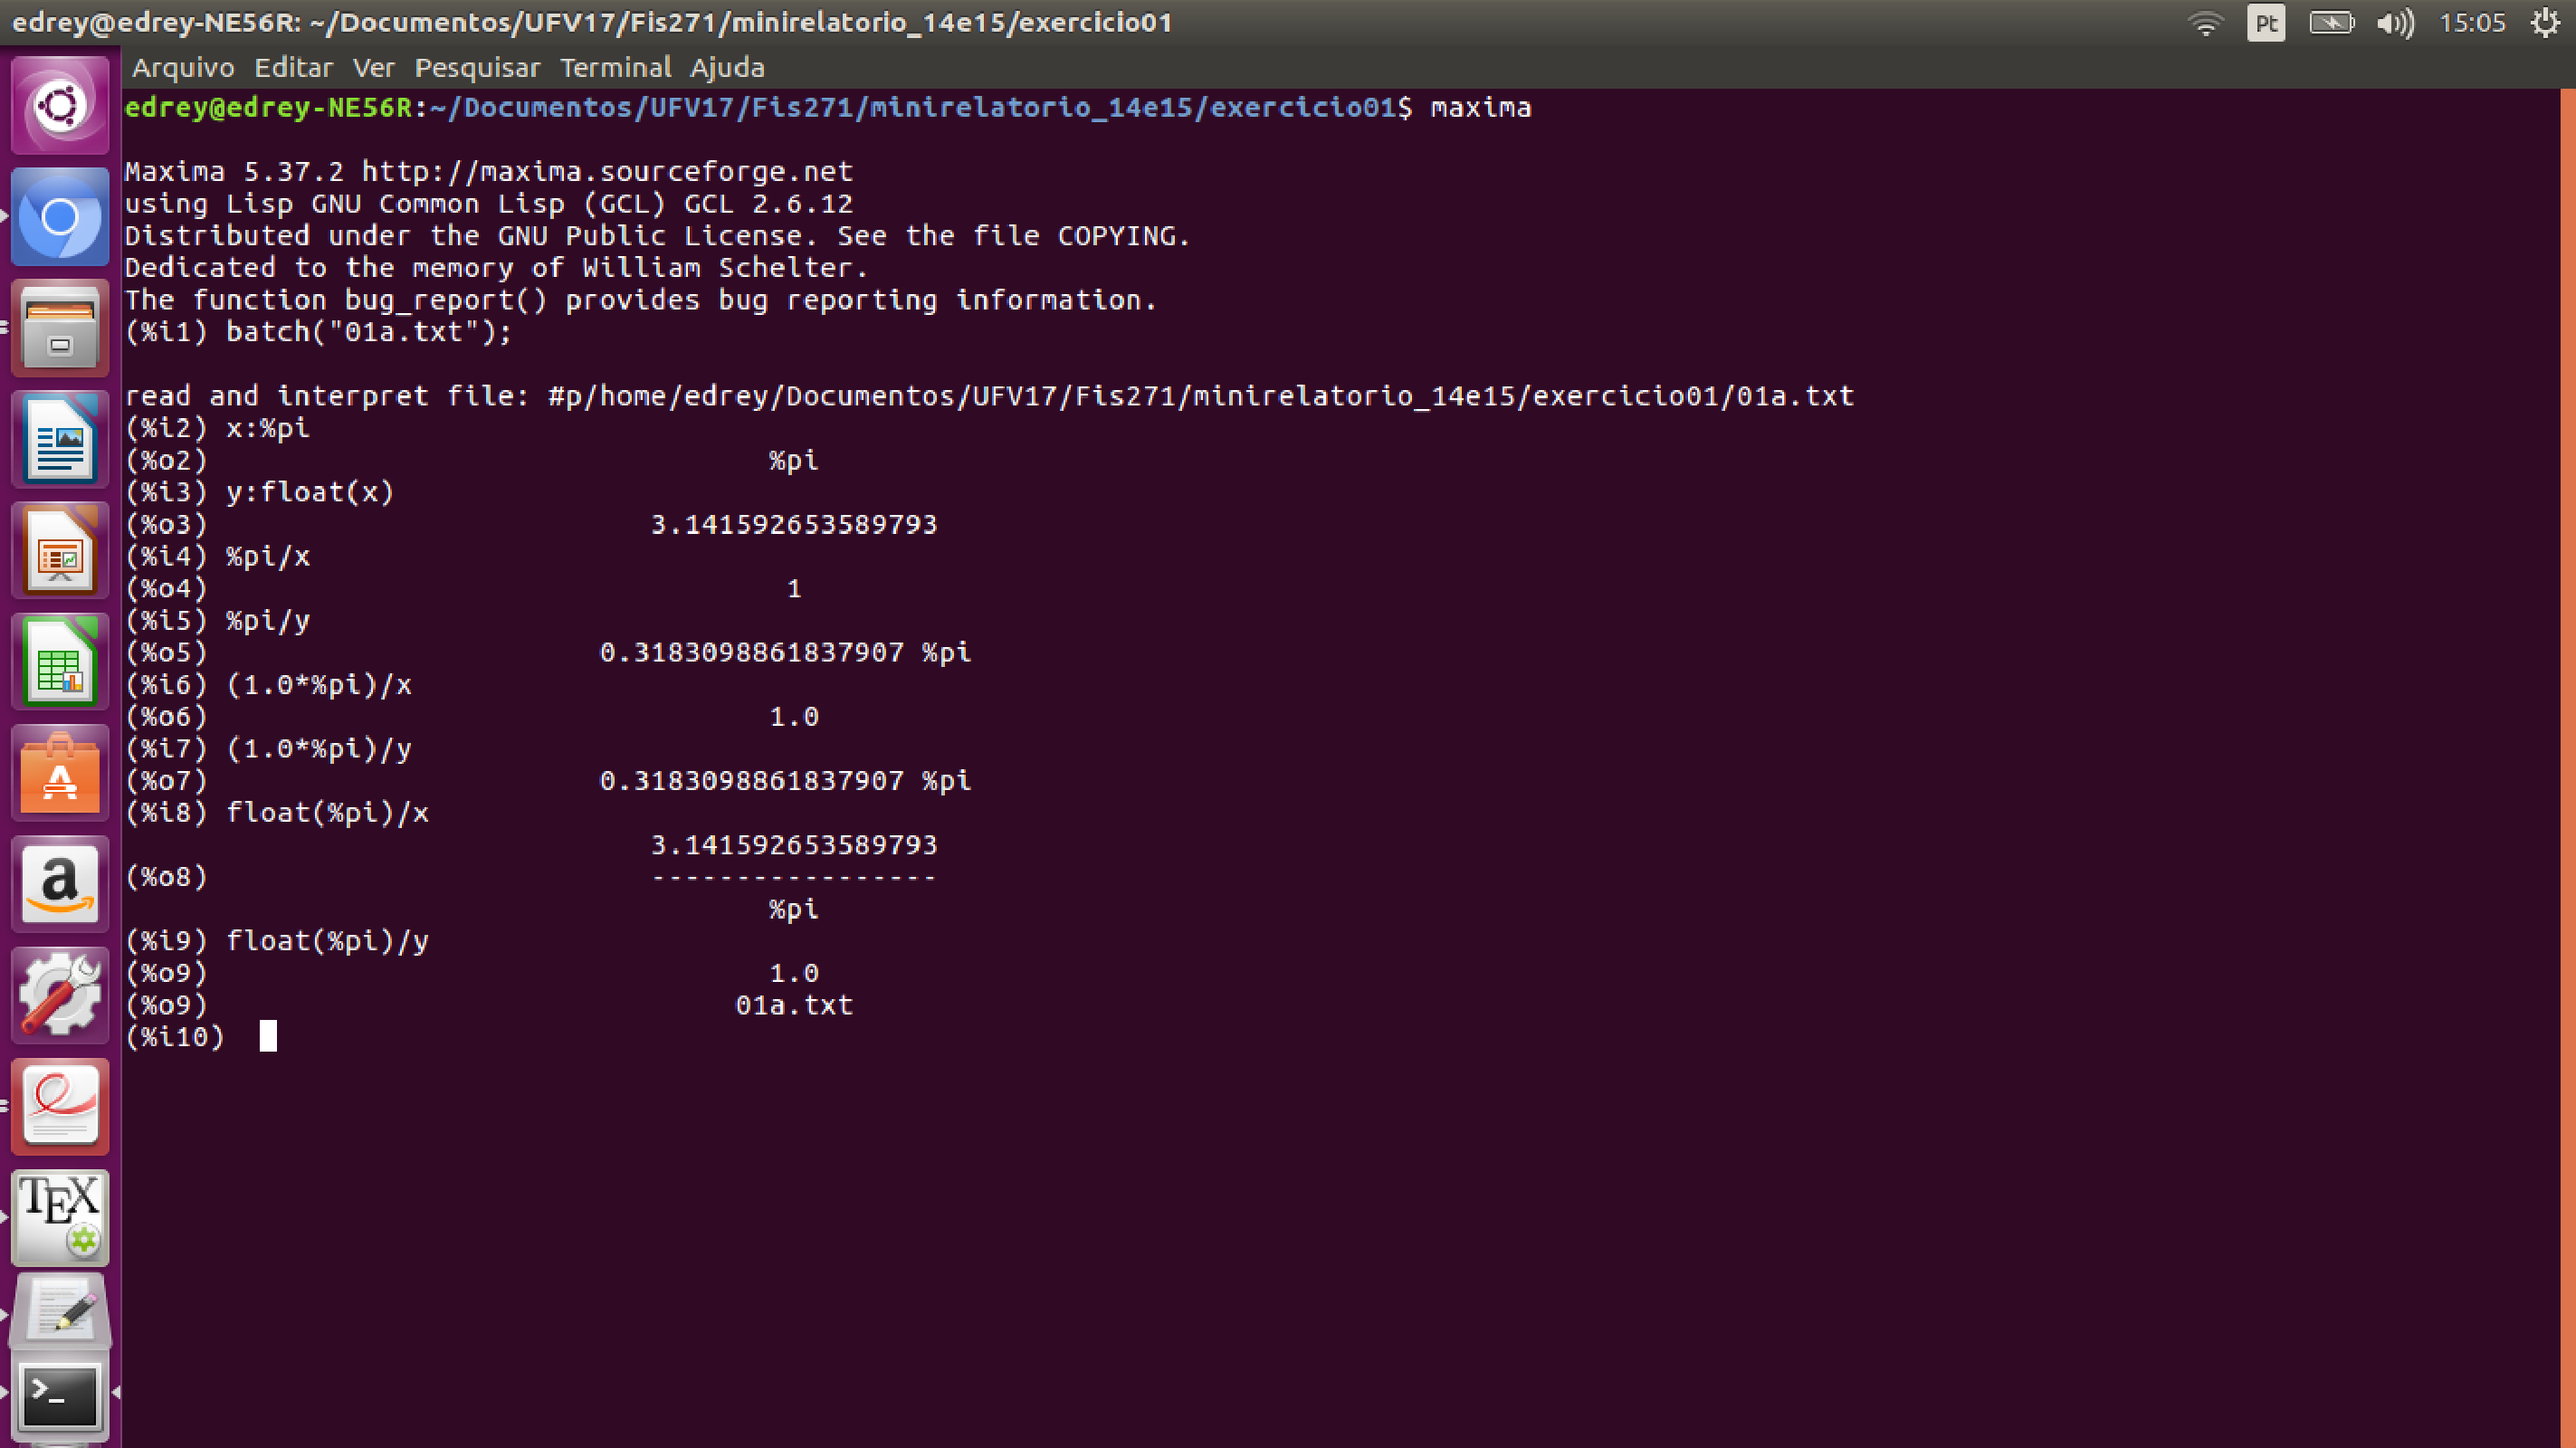
\includegraphics[width=0.50\textwidth]{01a.pdf}
\caption{A figura mostra os resultados encontrados após o programa rodar.}
\label{01a}
\end{figure}
\
\
\noindent{\bf Questão 1-b)} Nesse exercício o objetivo era verificar como o programa interpreta certos valores. Neste caso atribuimos os seguintes valores $z:\%e^(-1)$ e $w:\%e^(-1.0)$. z é interpretado como um valor algébrico, enquando w é interpretado como um número. Os valores foram operados como mostra a figura \ref{01b}. quando fazemos a multiplicação e*a o valor obtido é 1. Quando fazemos a multiplicação e*w encontramos um número multiplicando e, um número por um valor algébrico. Depois o comando float foi utilizado na multiplicação como pode ser observado na figura.

\begin{figure}[h]
\centering
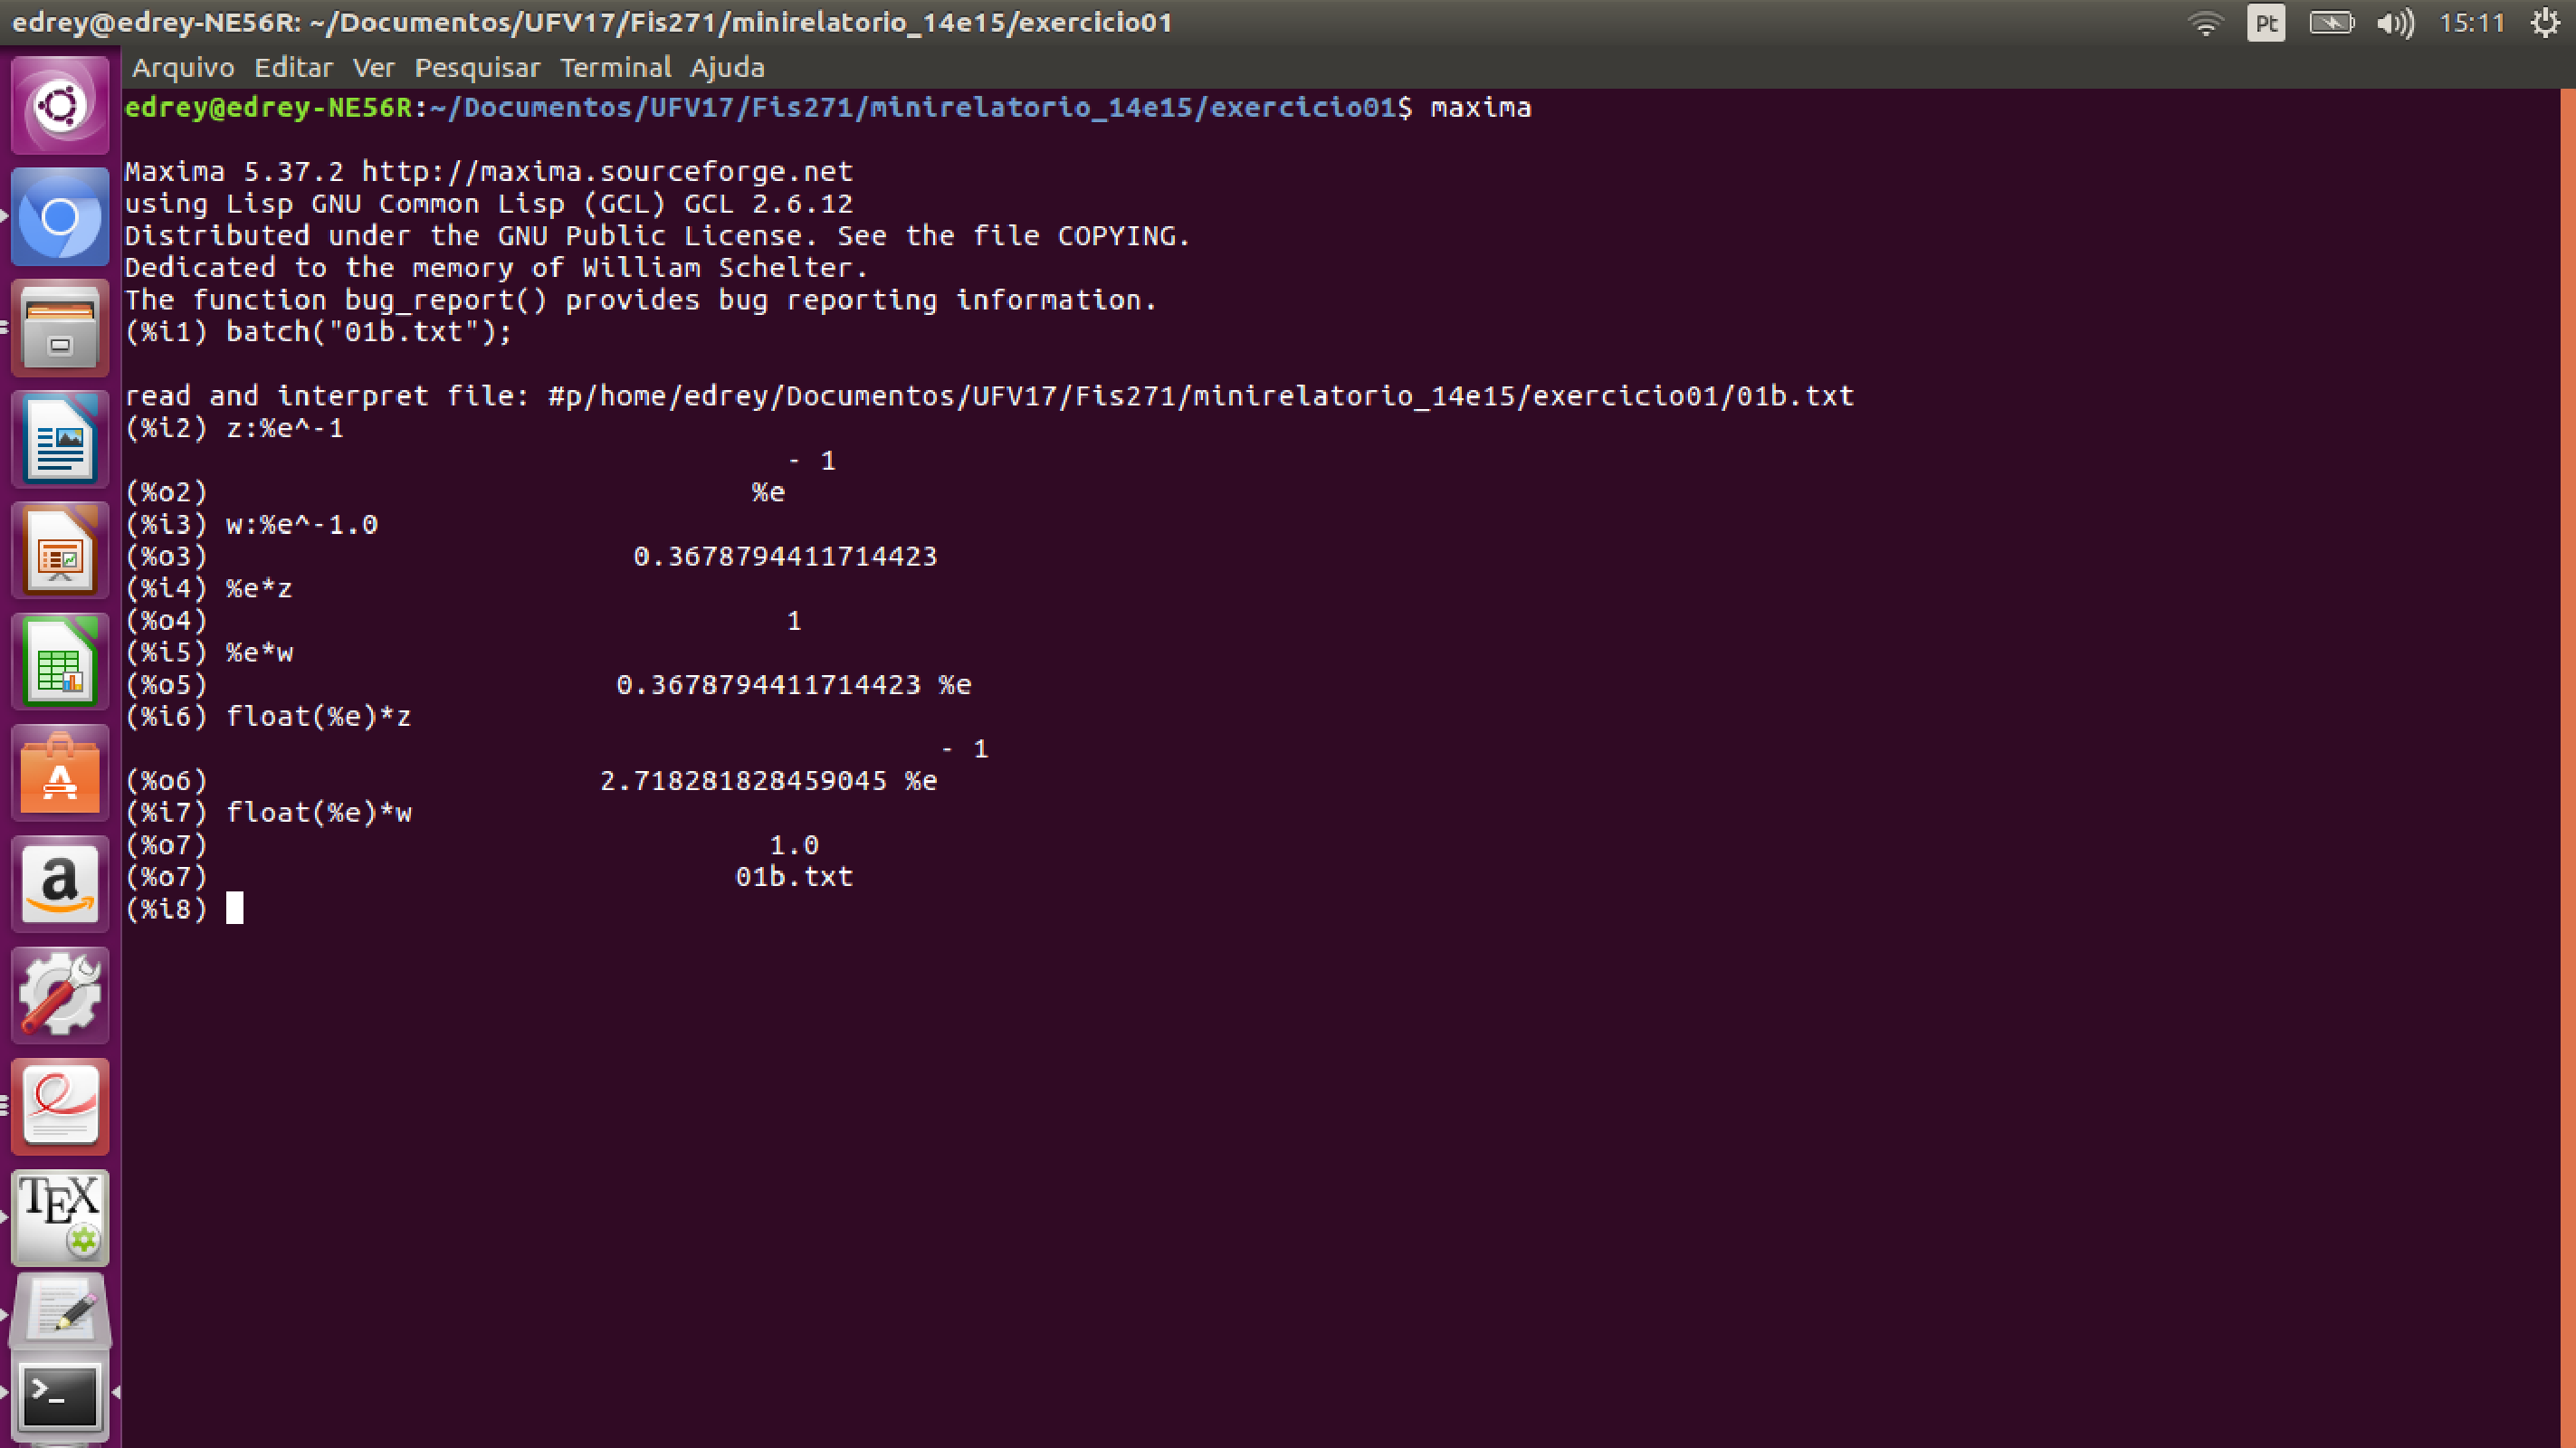
\includegraphics[width=0.50\textwidth]{01b.pdf}
\caption{A figura mostra os resultados encontrados após o programa rodar.}
\label{01b}
\end{figure}
\
\noindent{\bf Questão 1-c)} Foram atribuídos os valores a:411 e b:548, e depois foi feita a razão entre a e b de dois modos. O primeiro fazendo $c:a/b$ depois colocando a e b no comando float e fazendo a divisão como pode ser visto na figura \ref{01c}. E depois conhecer o comando rationalize que pega um valor decimal e o transforma em fração.

\begin{figure}[h]
\centering
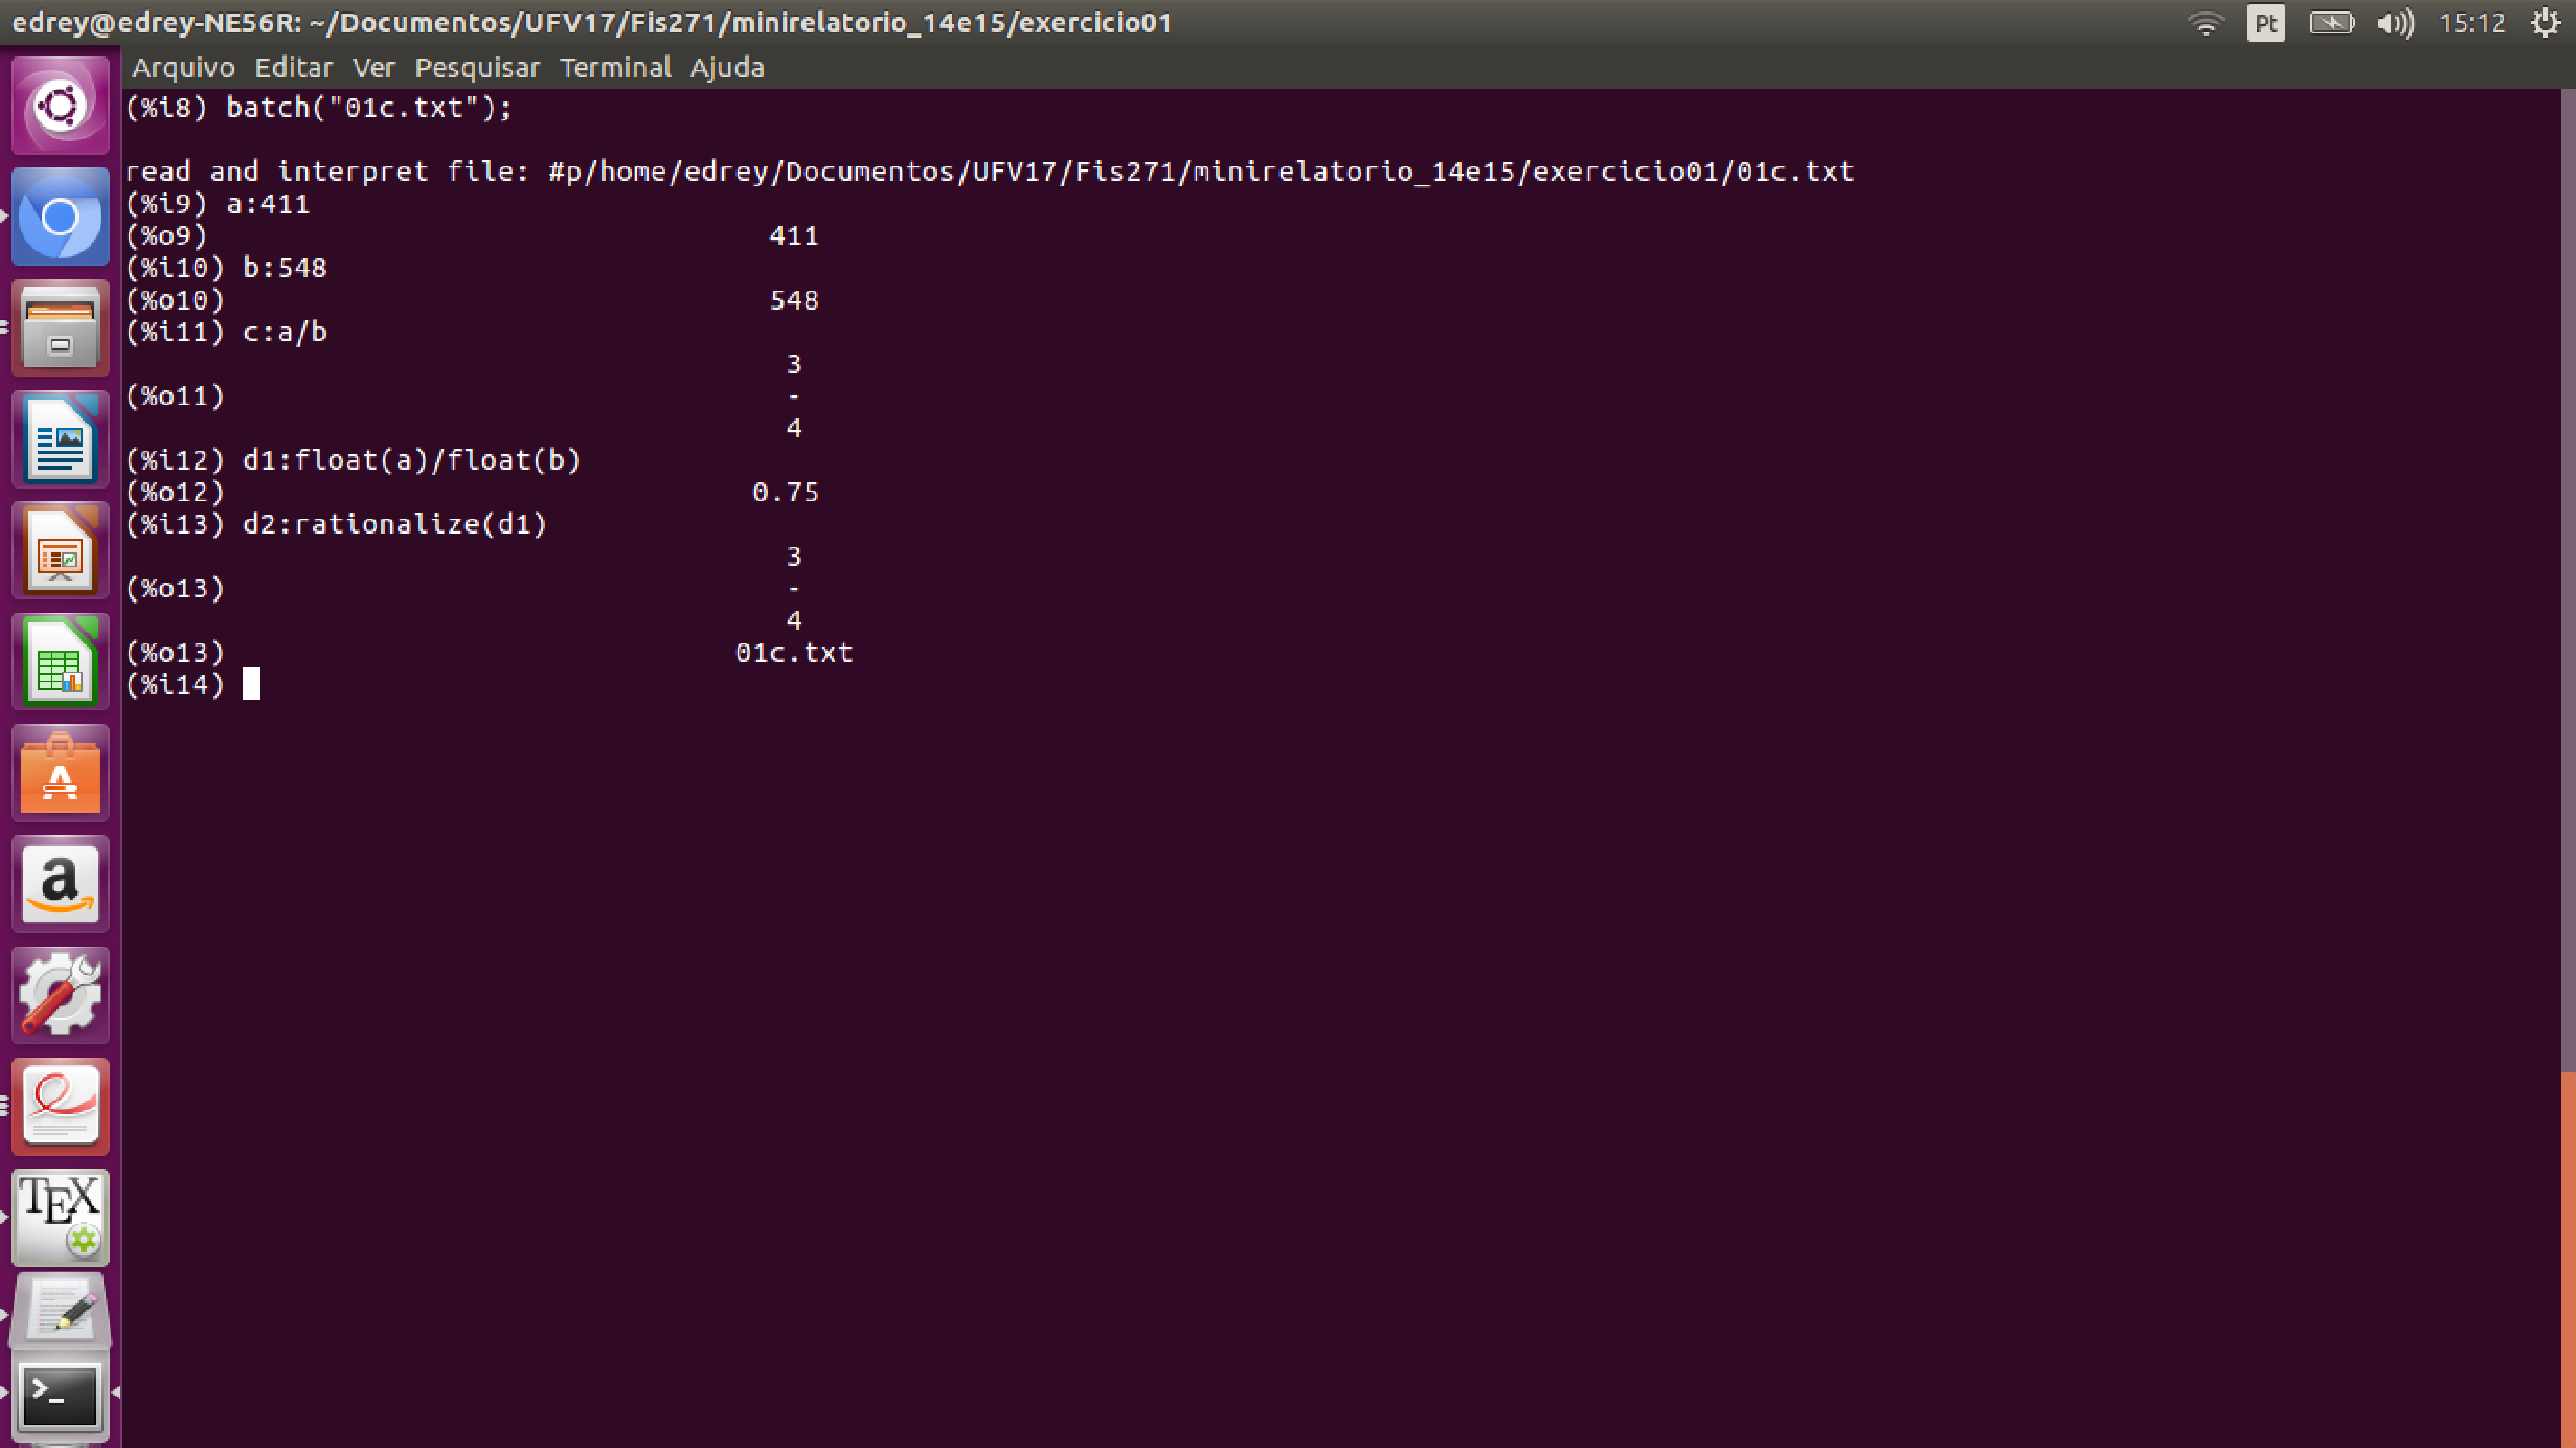
\includegraphics[width=0.50\textwidth]{01c.pdf}
\caption{A figura mostra os resultados encontrados após o programa rodar.}
\label{01c}
\end{figure}
\
\noindent{\bf Questão 1-d)} Nesse exercício o o roteiro é parecido com o anterior porém mudando os valores de a e b como mostra a figura \ref{01d}. Acredito que o comando rationalize não volta no valor c por questões de precisão do programa.

\begin{figure}[h]
\centering
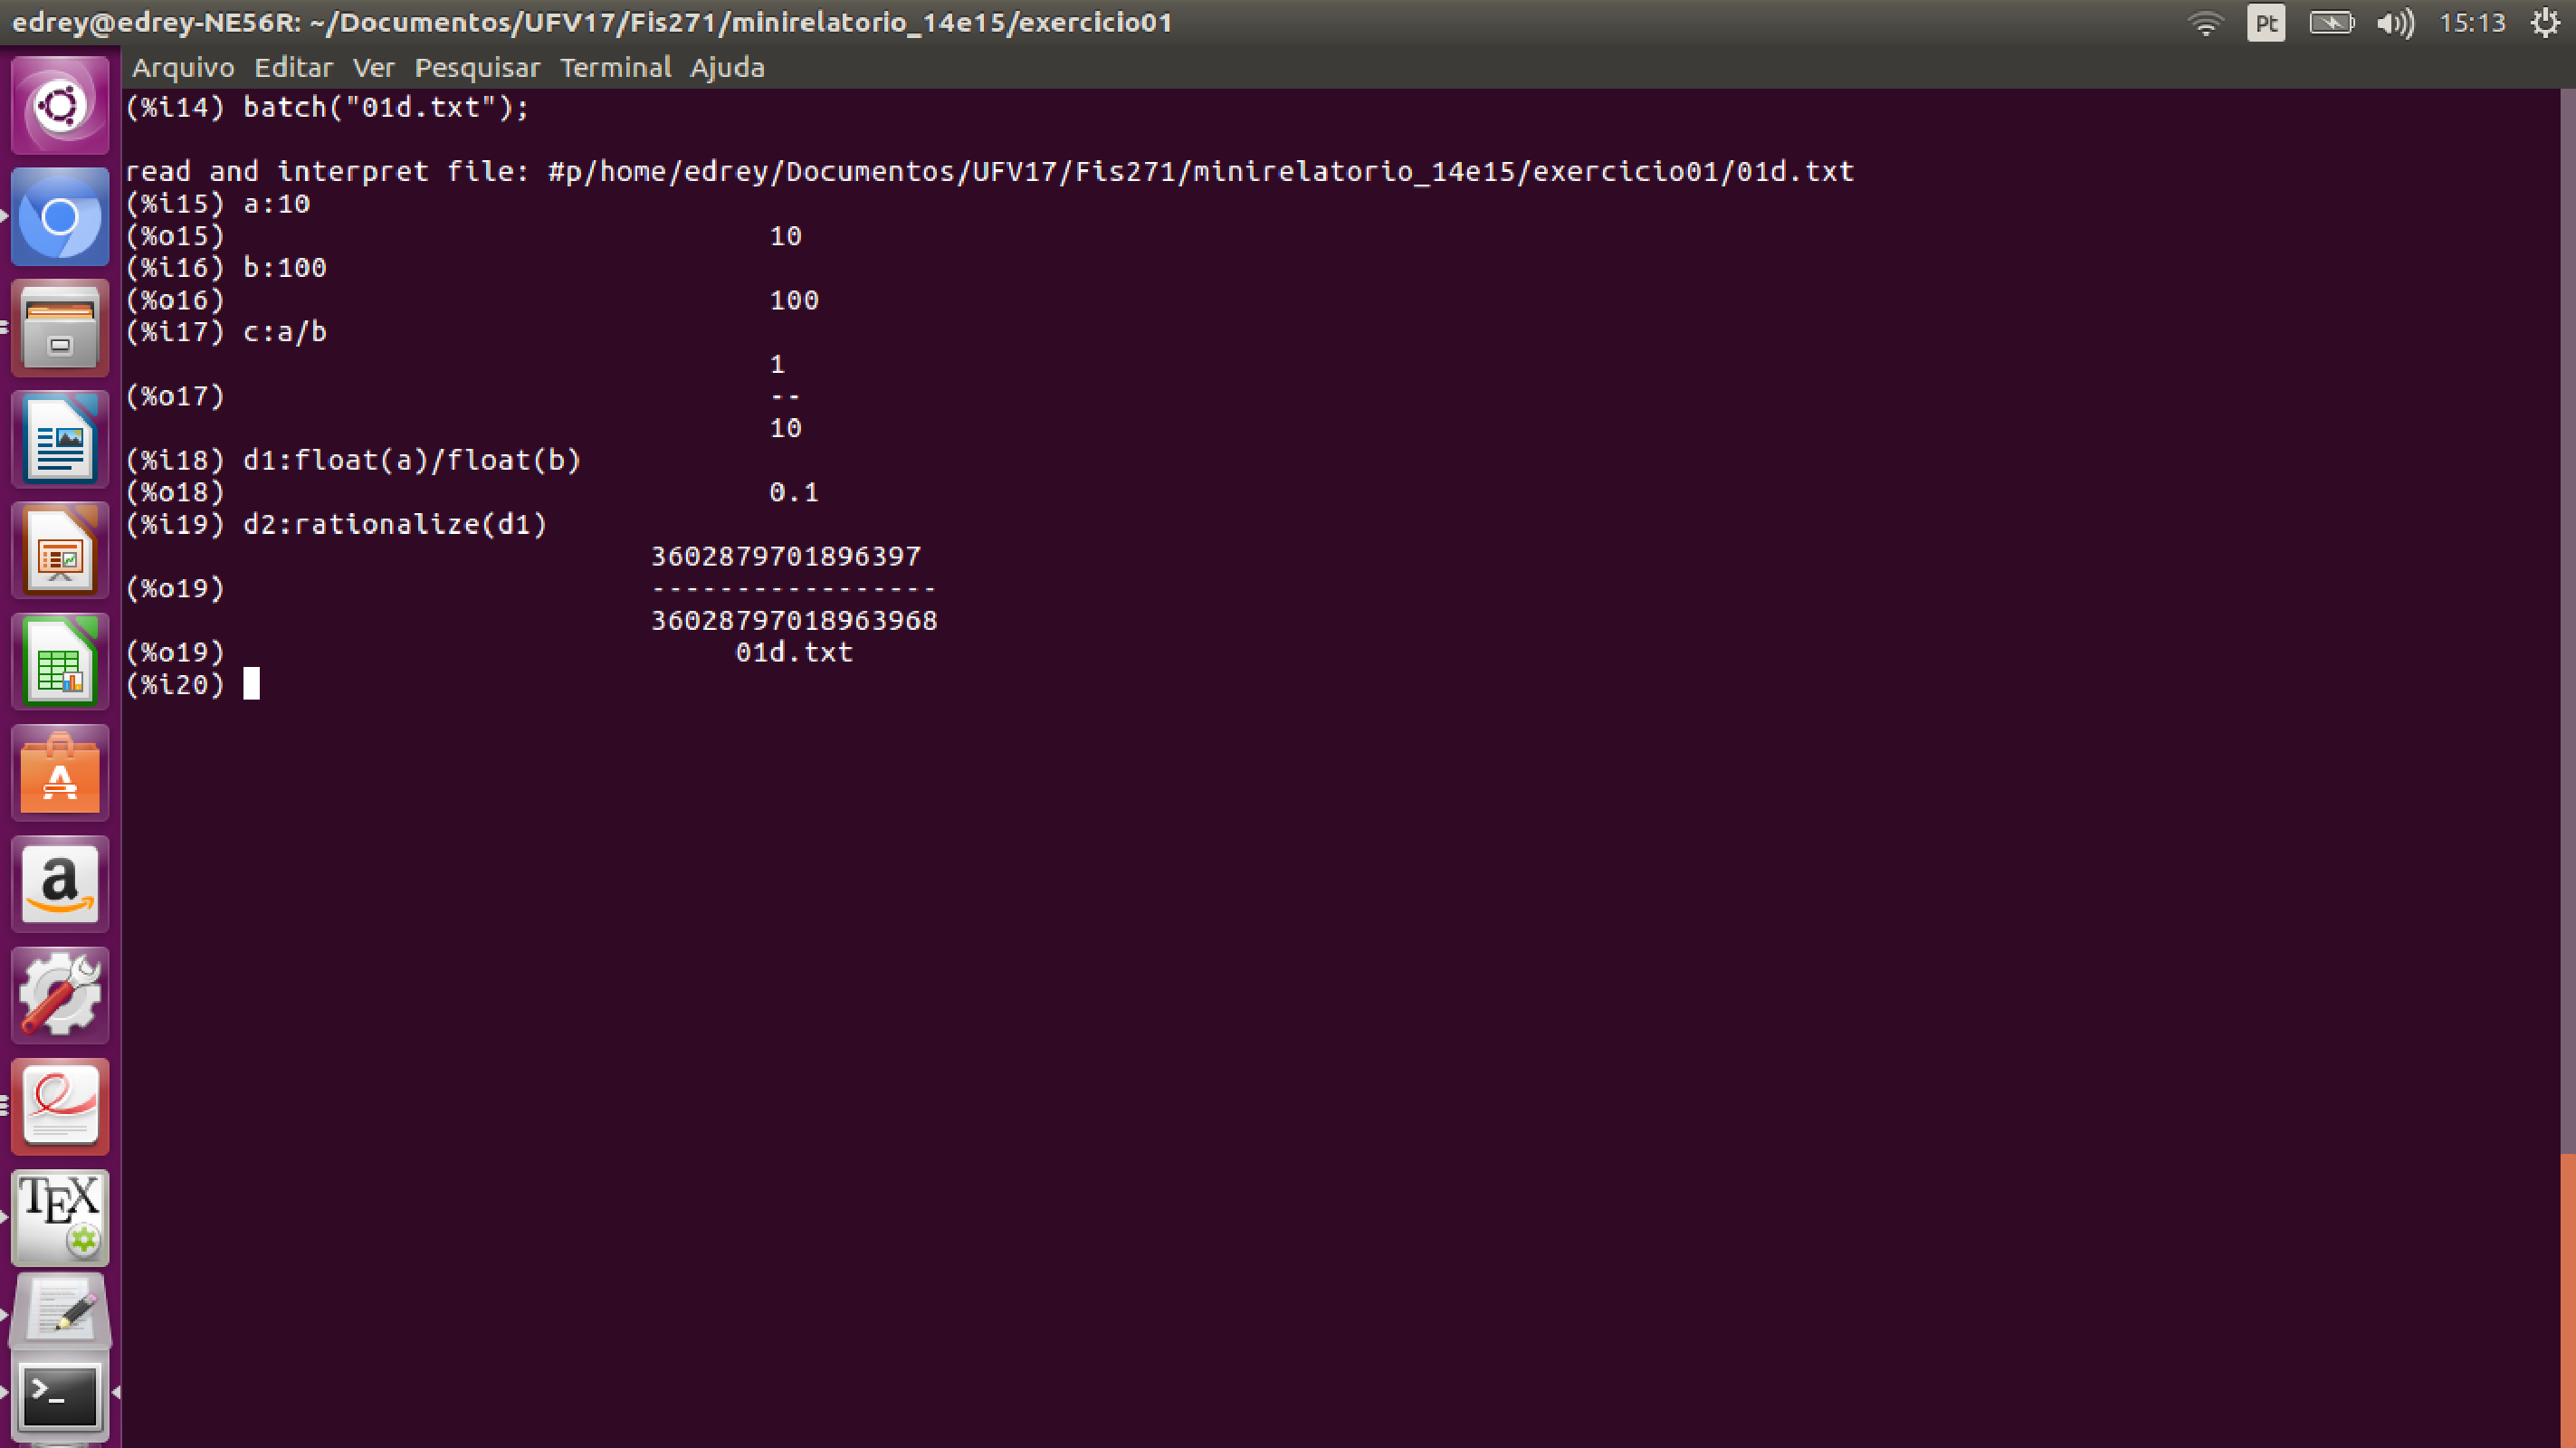
\includegraphics[width=0.50\textwidth]{01d.pdf}
\caption{A figura mostra os resultados encontrados após o programa rodar.}
\label{01d}
\end{figure}
\
\noindent{\bf Questão 1-e) \& f)} Nesses exercícios foram usados os comandos limit e derivative e os resultados estão mostrados na figura \ref{01ef}.
\
\begin{figure}[h]
\centering
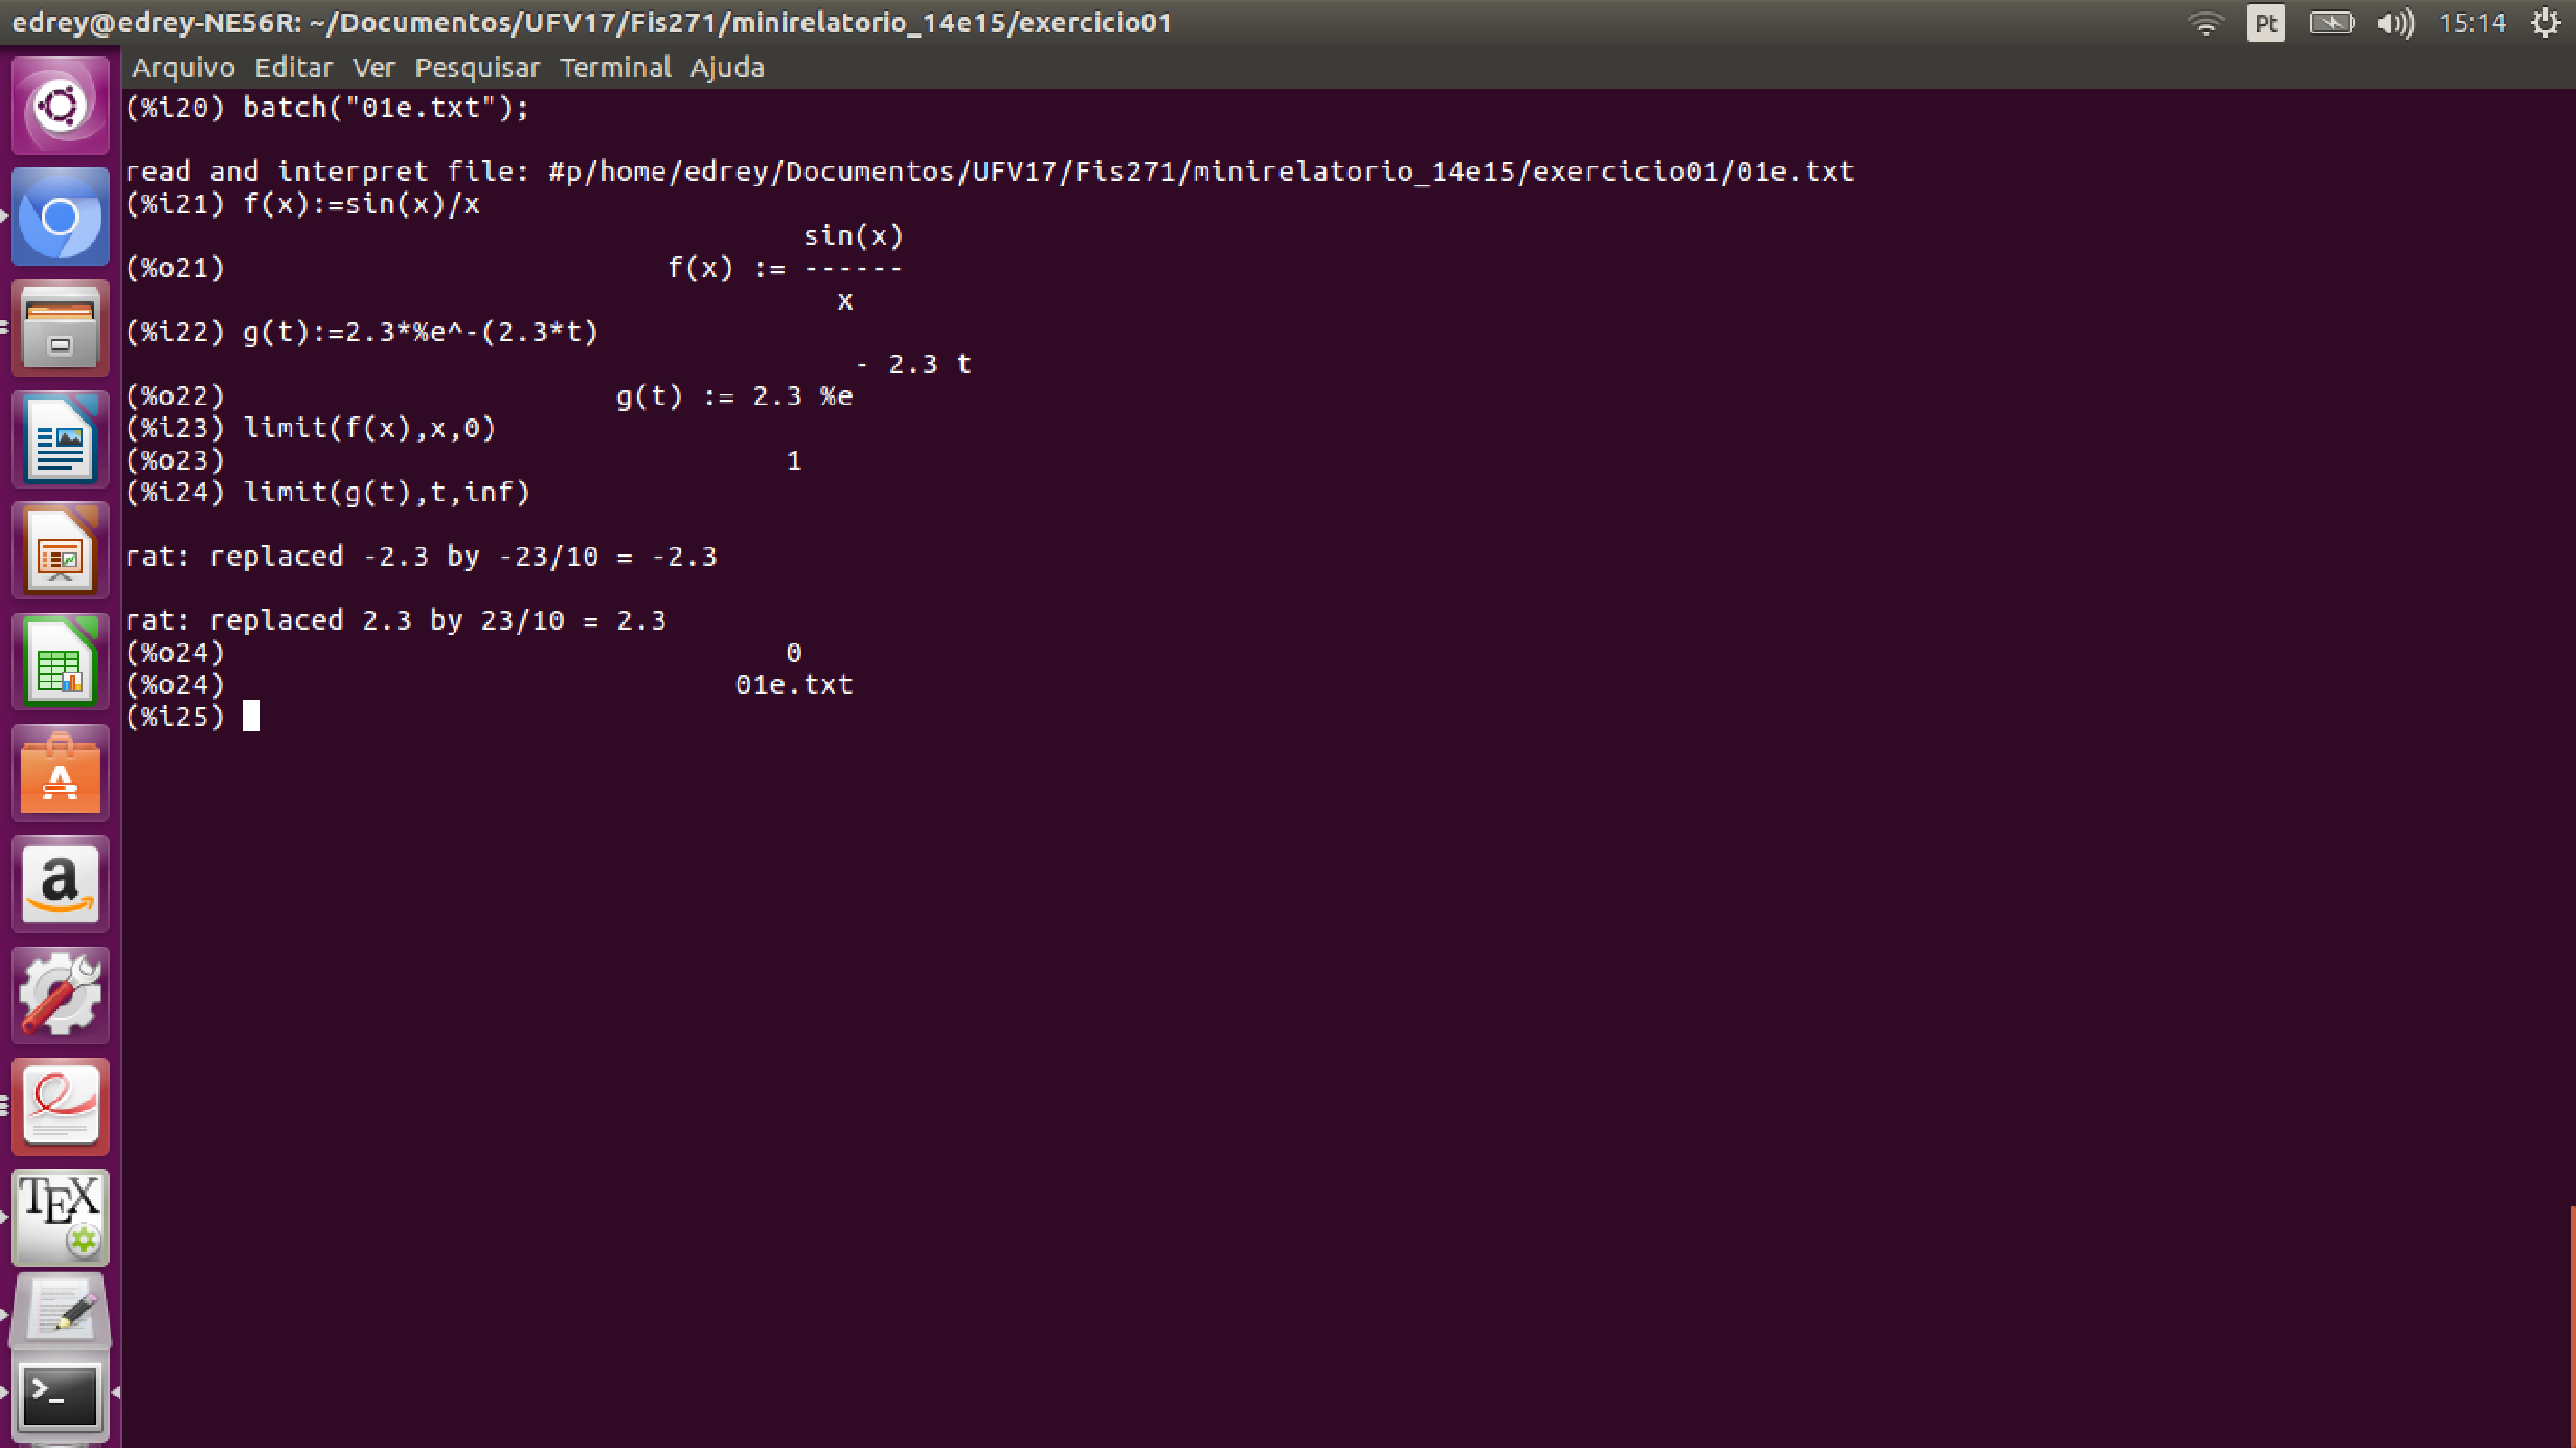
\includegraphics[width=0.30\textwidth]{01e.pdf}
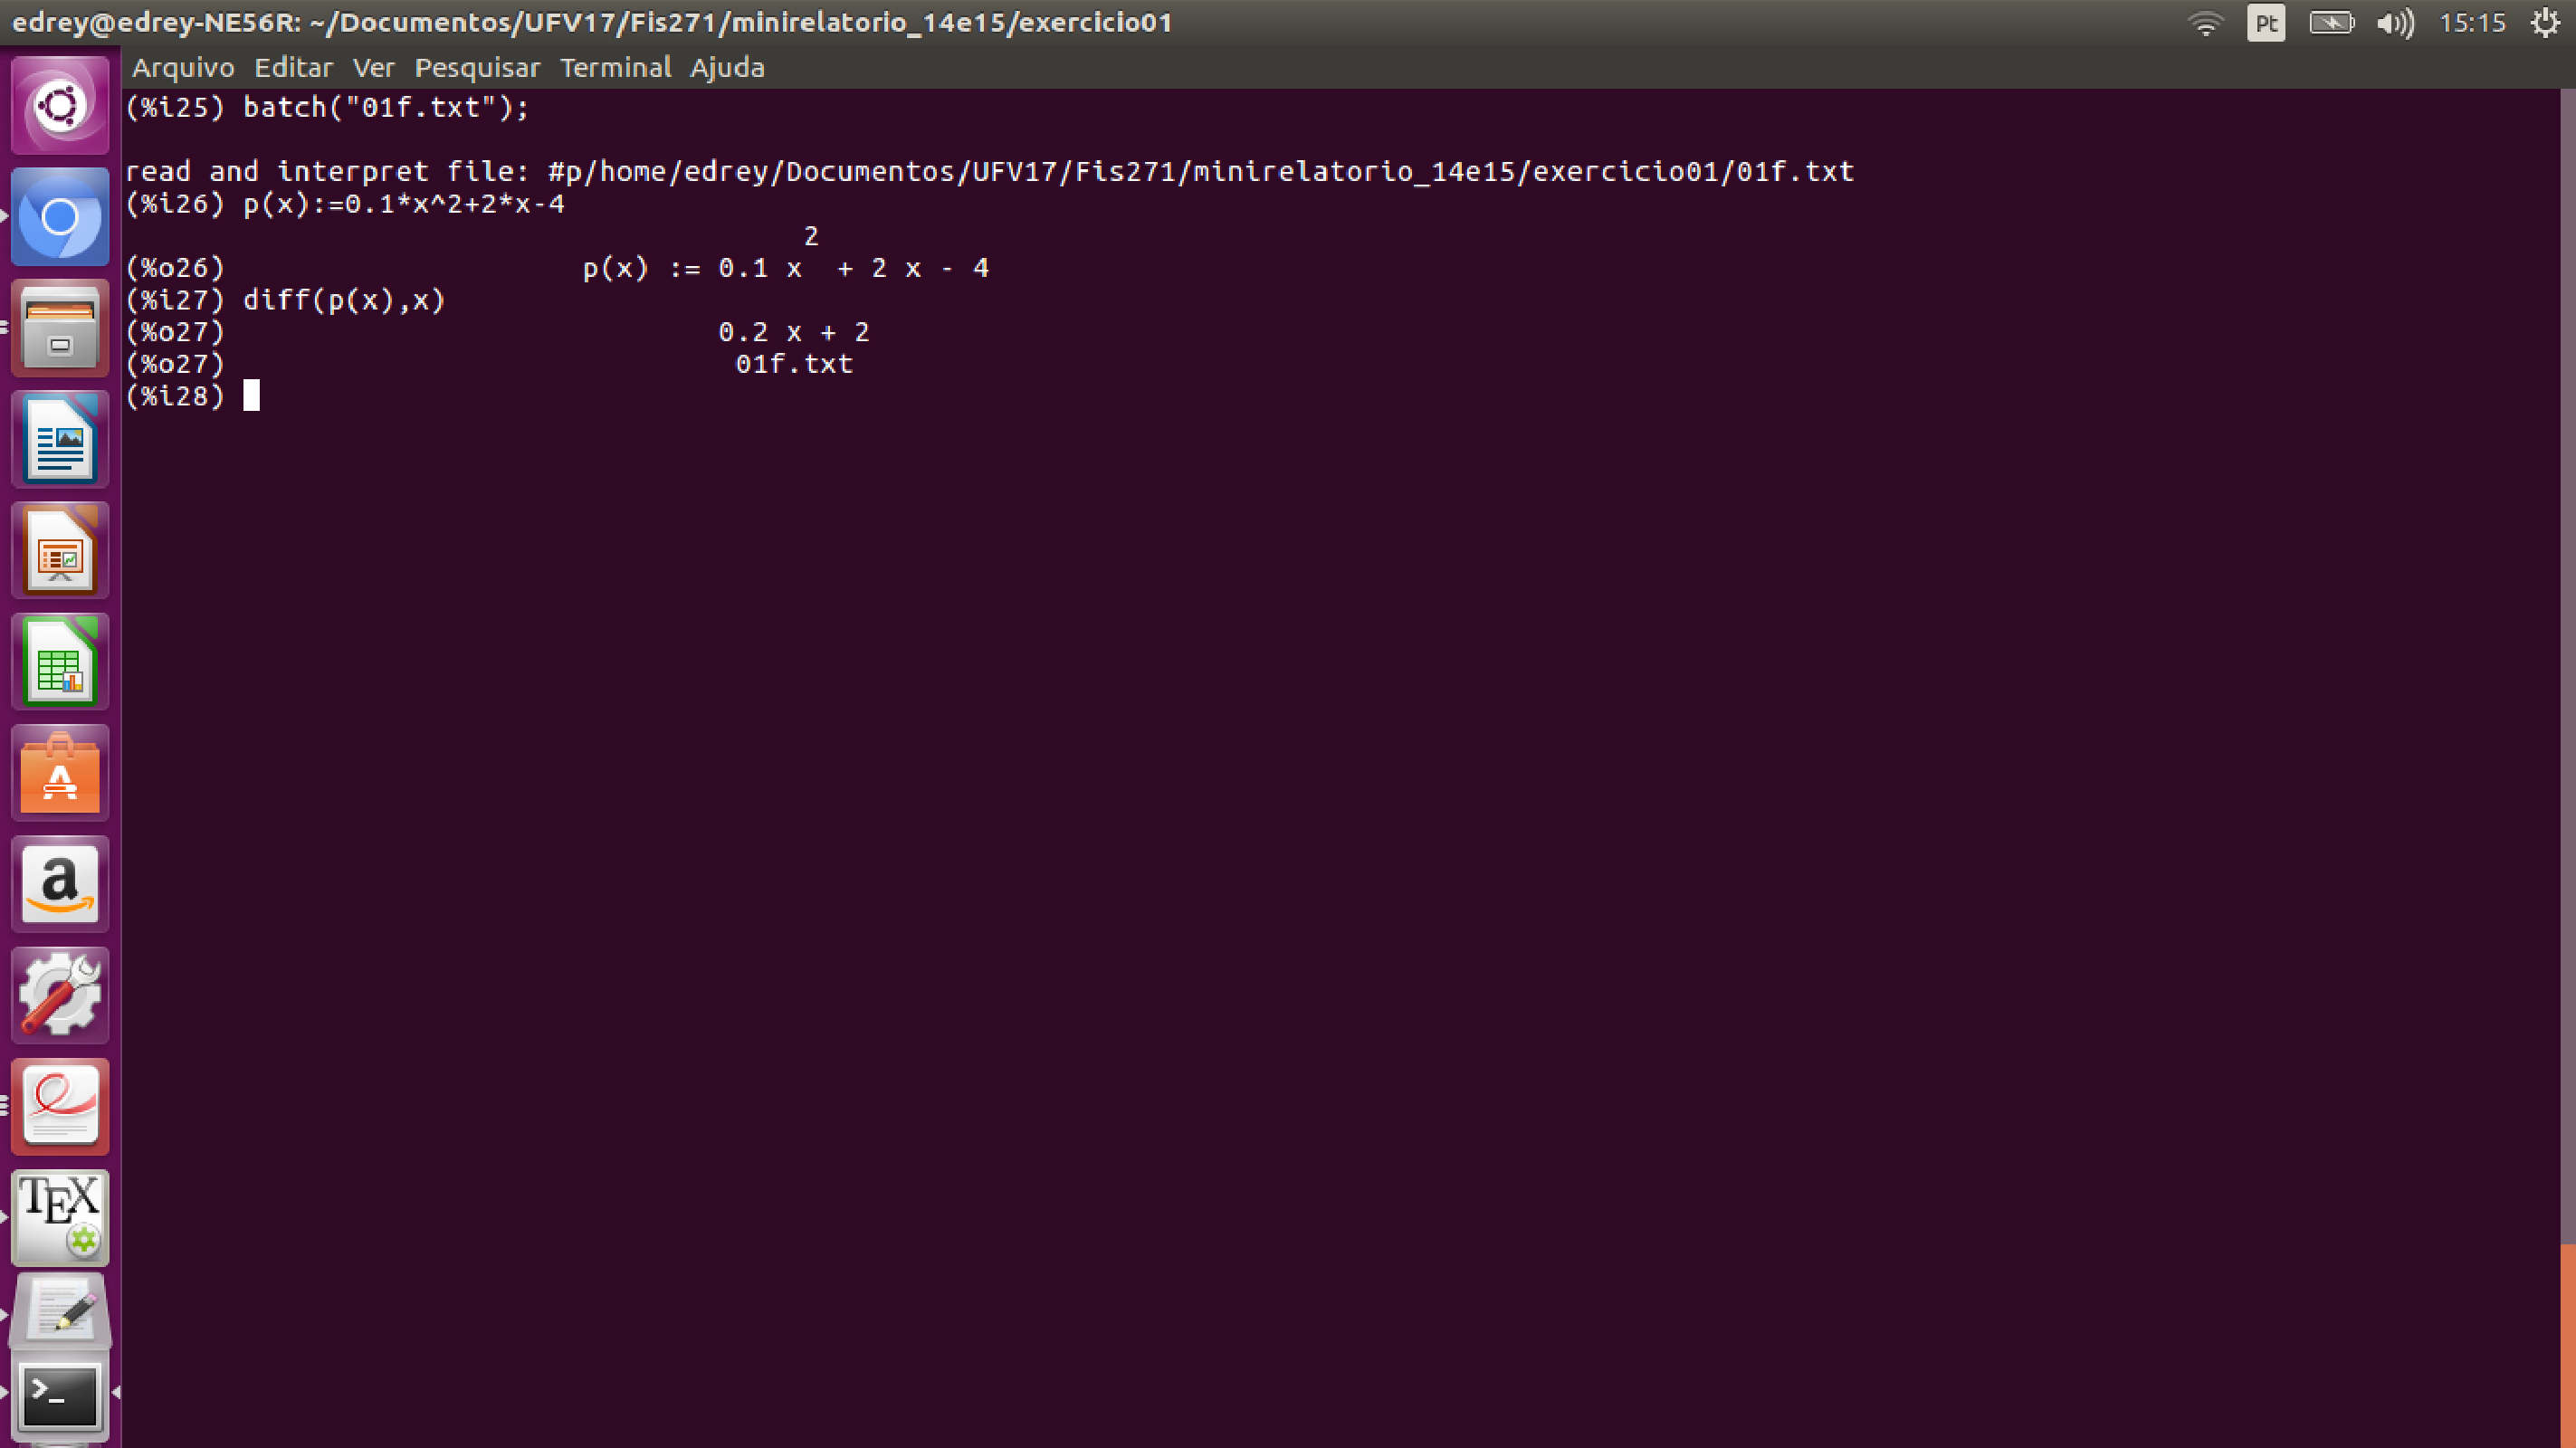
\includegraphics[width=0.30\textwidth]{01f.pdf}
\caption{A figura mostra os resultados encontrados após o programa rodar.}
\label{01ef}
\end{figure}
\

\noindent{\bf Questão 2-} Nesse exercícios o objetivo era plotar um gráfico de van der Waals para as temperaturas $0.9T_{c}$,$T_{c}$ e $1.1T_{c}$ utilizando o comando plot2d. Plotamos então os seguintes gráficos na figura \ref{02}.\\
\begin{eqnarray}
P_{1}(v) &=& \frac{2R(0.9T_{c})}{v-2b}-\frac{4a}{v^{2}}\\
P_{2}(v) &=& \frac{2RT_{c}}{v-2b}-\frac{4a}{v^{2}}\\
P_{3}(v) &=& \frac{2R(1.1T_{c})}{v-2b}-\frac{4a}{v^{2}}
\end{eqnarray}
\
Sendo R a constante dos gases ideais, e a e b constantes associadas ao gás de van der Walls.


\
\begin{figure}[h]
\centering
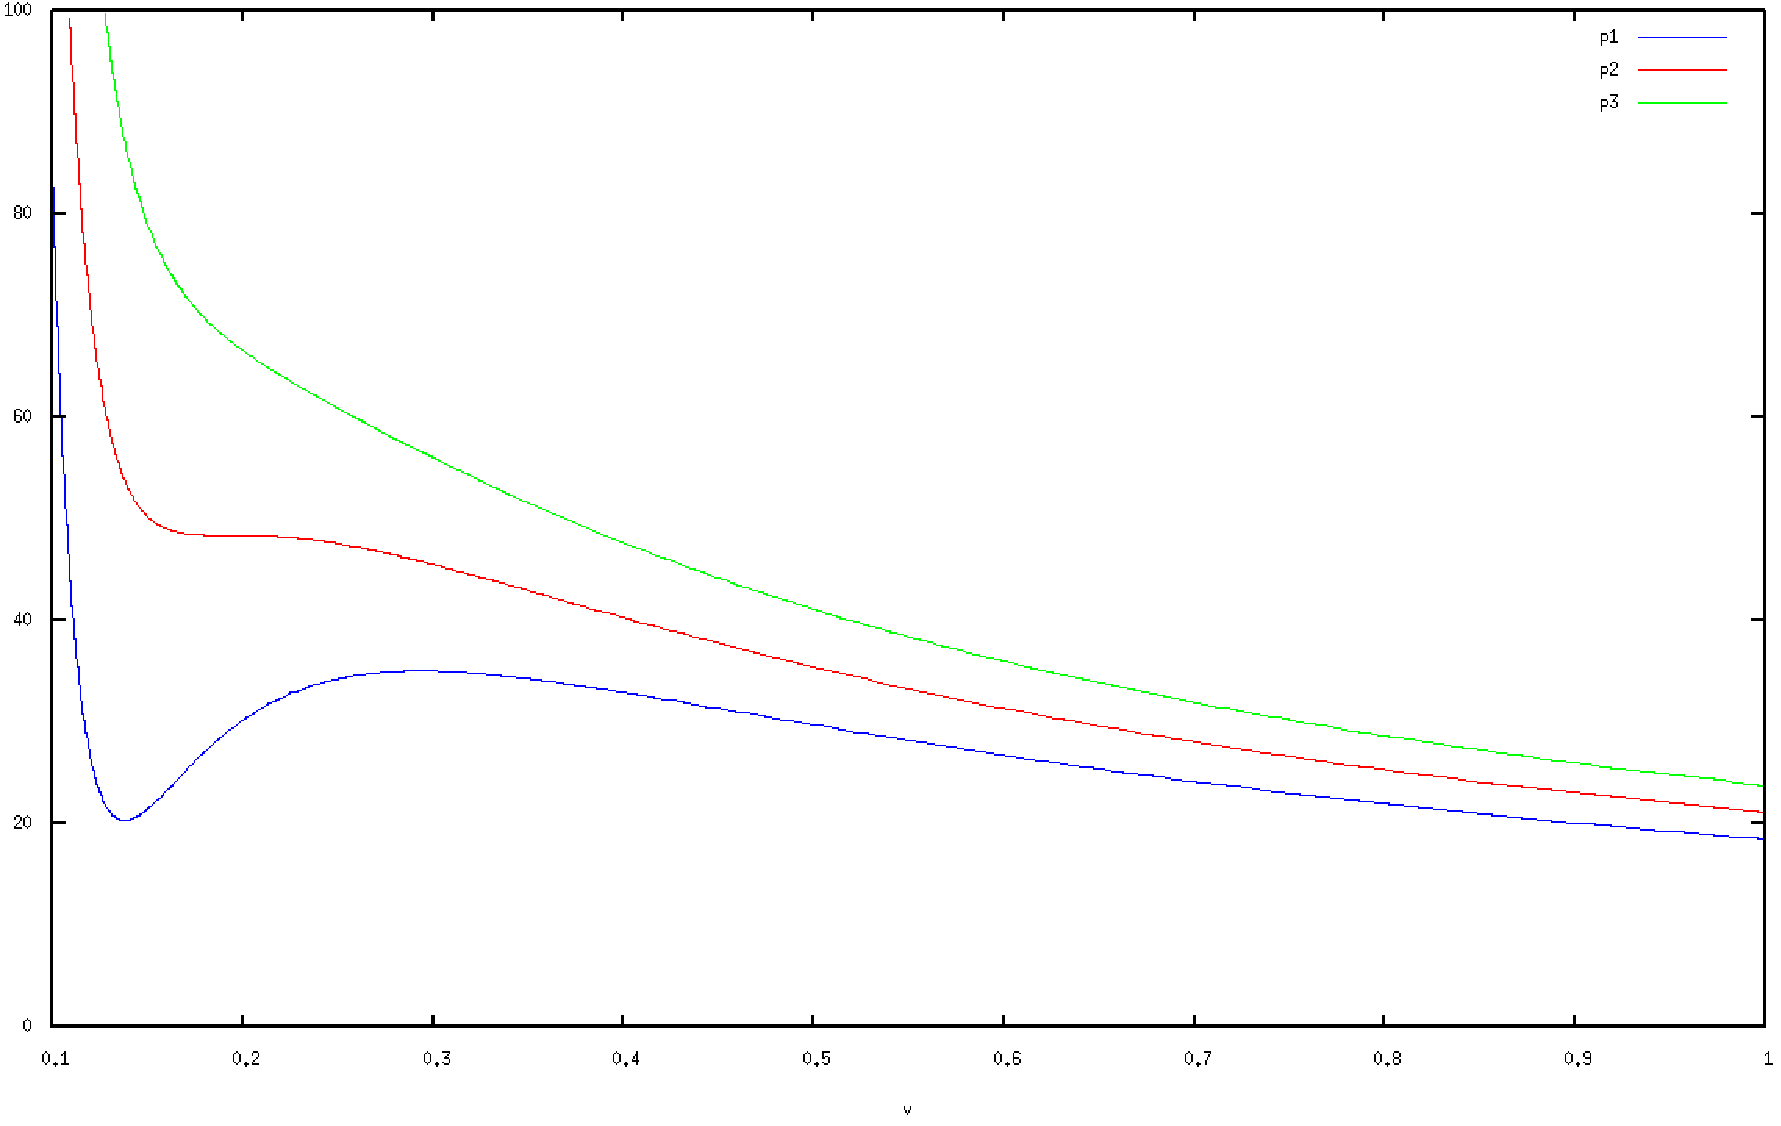
\includegraphics[width=0.30\textwidth]{02.pdf}
\caption{A figura mostra o gŕáfico de P(V) para o gás de van der Waals em várias temperaturas.}
\label{02}
\end{figure}
\
\noindent{\bf Questão 3-a)} Nesse exercício o objetivo é utilizar o comando plot2d para plotar a função $x(t)=A\cos(\omega t+q)$. Sendo $A=1$,$\omega=1$ e $q=\dfrac{\pi}{2}$. O gráfico pode ser visto na figura \ref{03}.

\
\begin{figure}[h]
\centering
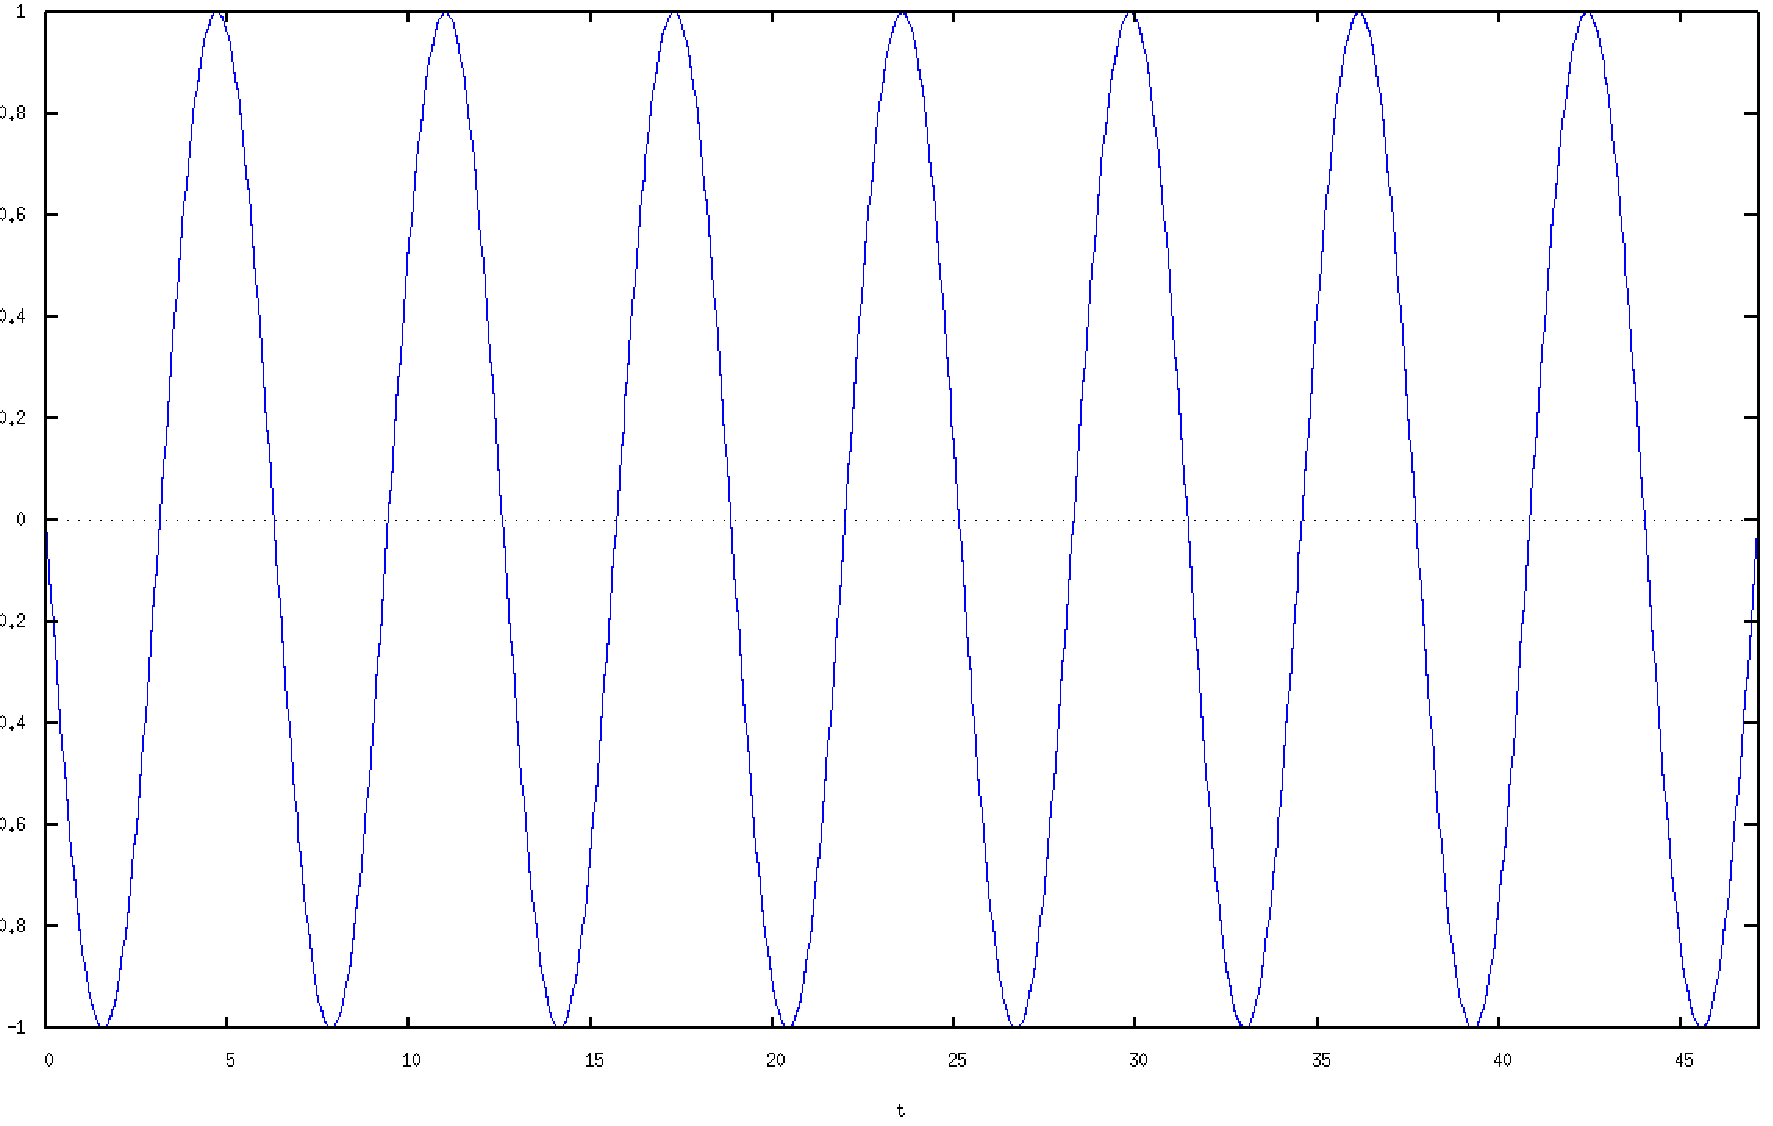
\includegraphics[width=0.30\textwidth]{03a.pdf}
\caption{A figura mostra o gráfico de $x(t)=\cos(t+\dfrac{\pi}{2})$.}
\label{03}
\end{figure}
\
\noindent{\bf Questão 3-b)} Nesse exercício foi usado o comando derivative duas vezes em $x(t)$ para encontrar $v(t)$e$a(t)$ e depois foram plotados os gráficos como é mostrado na figura \ref{03b}.

\
\begin{figure}[h]
\centering
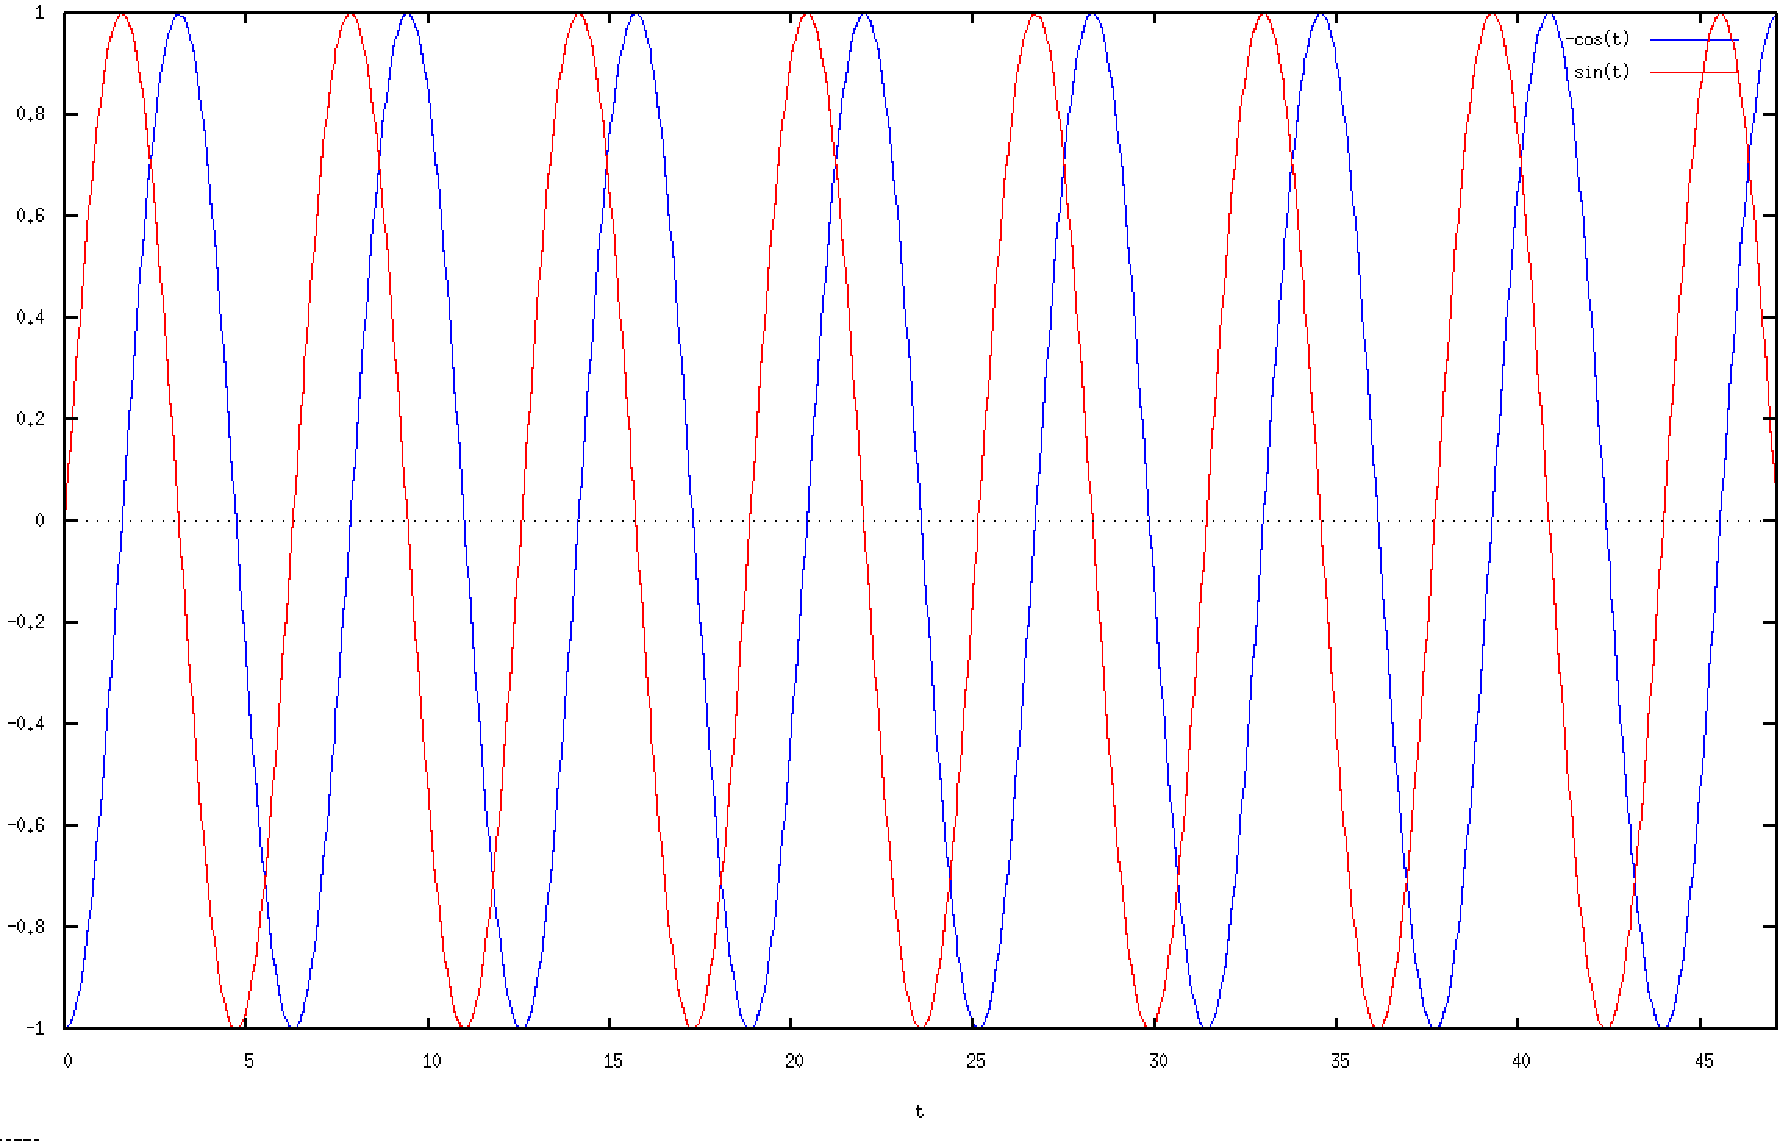
\includegraphics[width=0.30\textwidth]{03b.pdf}
\caption{A figura mostra na curva azul $v(t)$ e na curva vermelha $a(t)$.}
\label{03b}
\end{figure}
\

\noindent{\bf Questão 3-c)} Neste exercício integramos a(t) e comparamos o resultado u(t) dessa integral com v(t) encontrado em exercícios anteriores de modo que o gráfico está representado na figura \ref{03c}.

\
\begin{figure}[h]
\centering
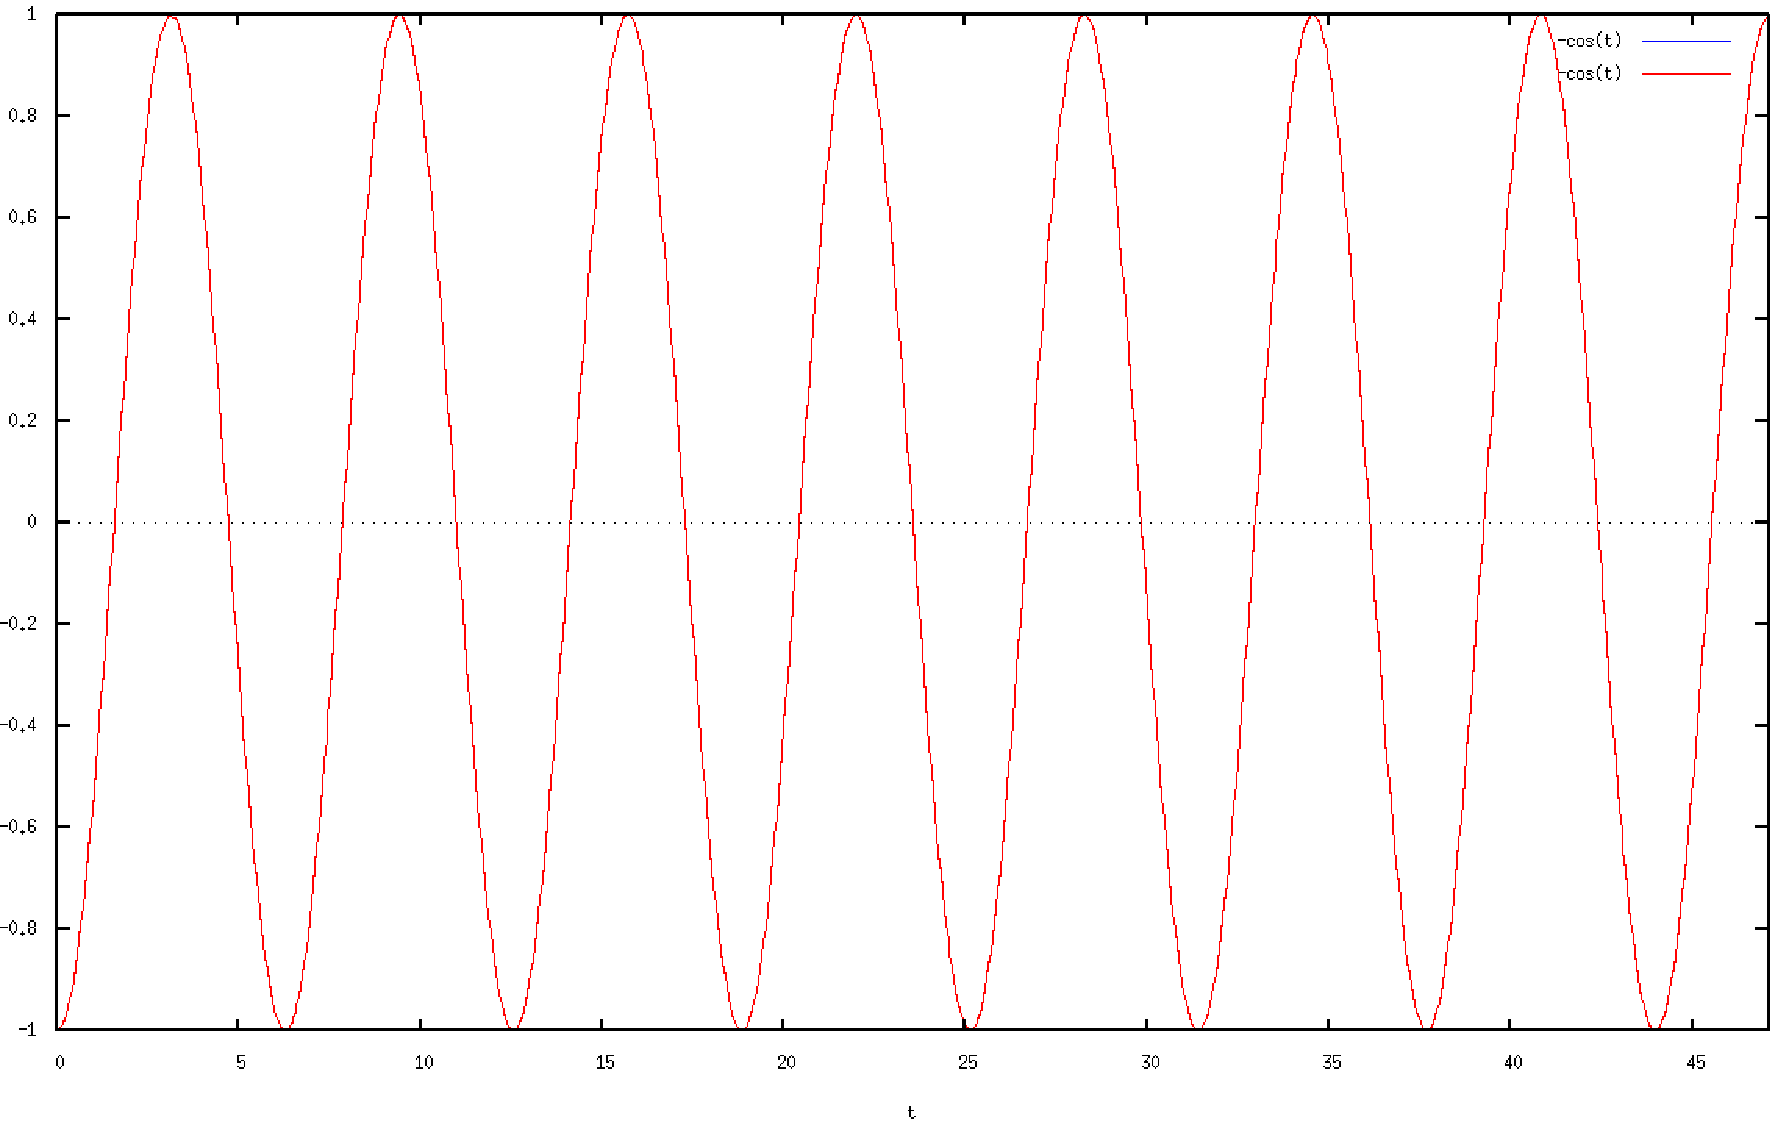
\includegraphics[width=0.30\textwidth]{03c.pdf}
\caption{A figura mostra os gráfico que estão super postos de u e v.}
\label{03c}
\end{figure}
\
\noindent{\bf Questão 3-d)} Neste exercício a idéia é utilizar a solução do oscilador de morse e derivar a velocidade e a aceleração e plotar os gráficos como mostra a figura 

\
\begin{figure}[h]
\centering
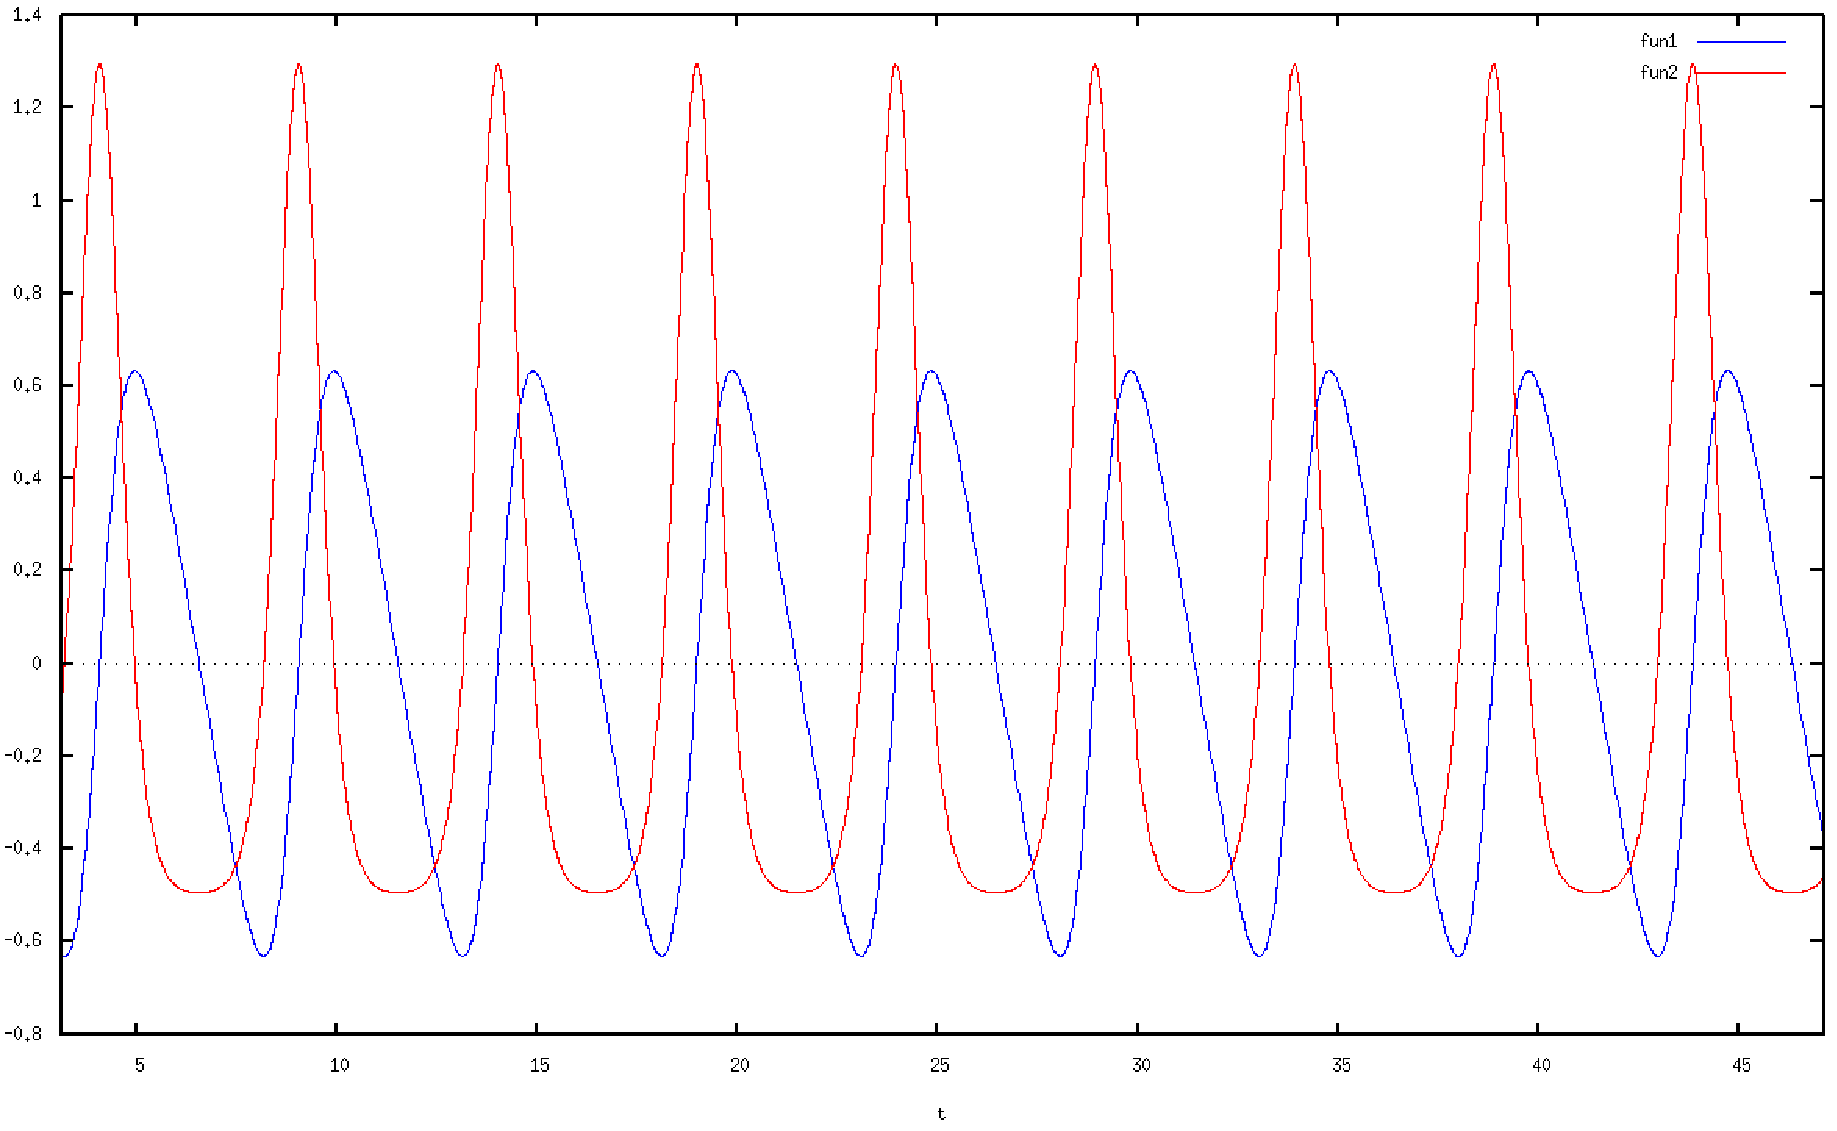
\includegraphics[width=0.30\textwidth]{03d.pdf}
\caption{O gráfico mostra a velocidade (curva vermelha) e a aceleração (curva azul) obtidas a partir da solução r(t) do oscilador de morse.}
\label{03d}
\end{figure}
\
\noindent{\bf Questão 4-)} Nesse exercícios tivemos que fazer o gŕafico da distribuição de energias e calcular o número de partículas depois de um gás passar pelo processo de evaporação. Nesse caso a distribuição de energia está disposta no gráfico da figura \ref{04}. E utilizanto a ferramenta de integração do maxima encontramos um valor para o número de partículas após a evaporação $N=1,84107654345791e^{-13}/\sqrt{\pi}$
\
\begin{figure}[h]
\centering
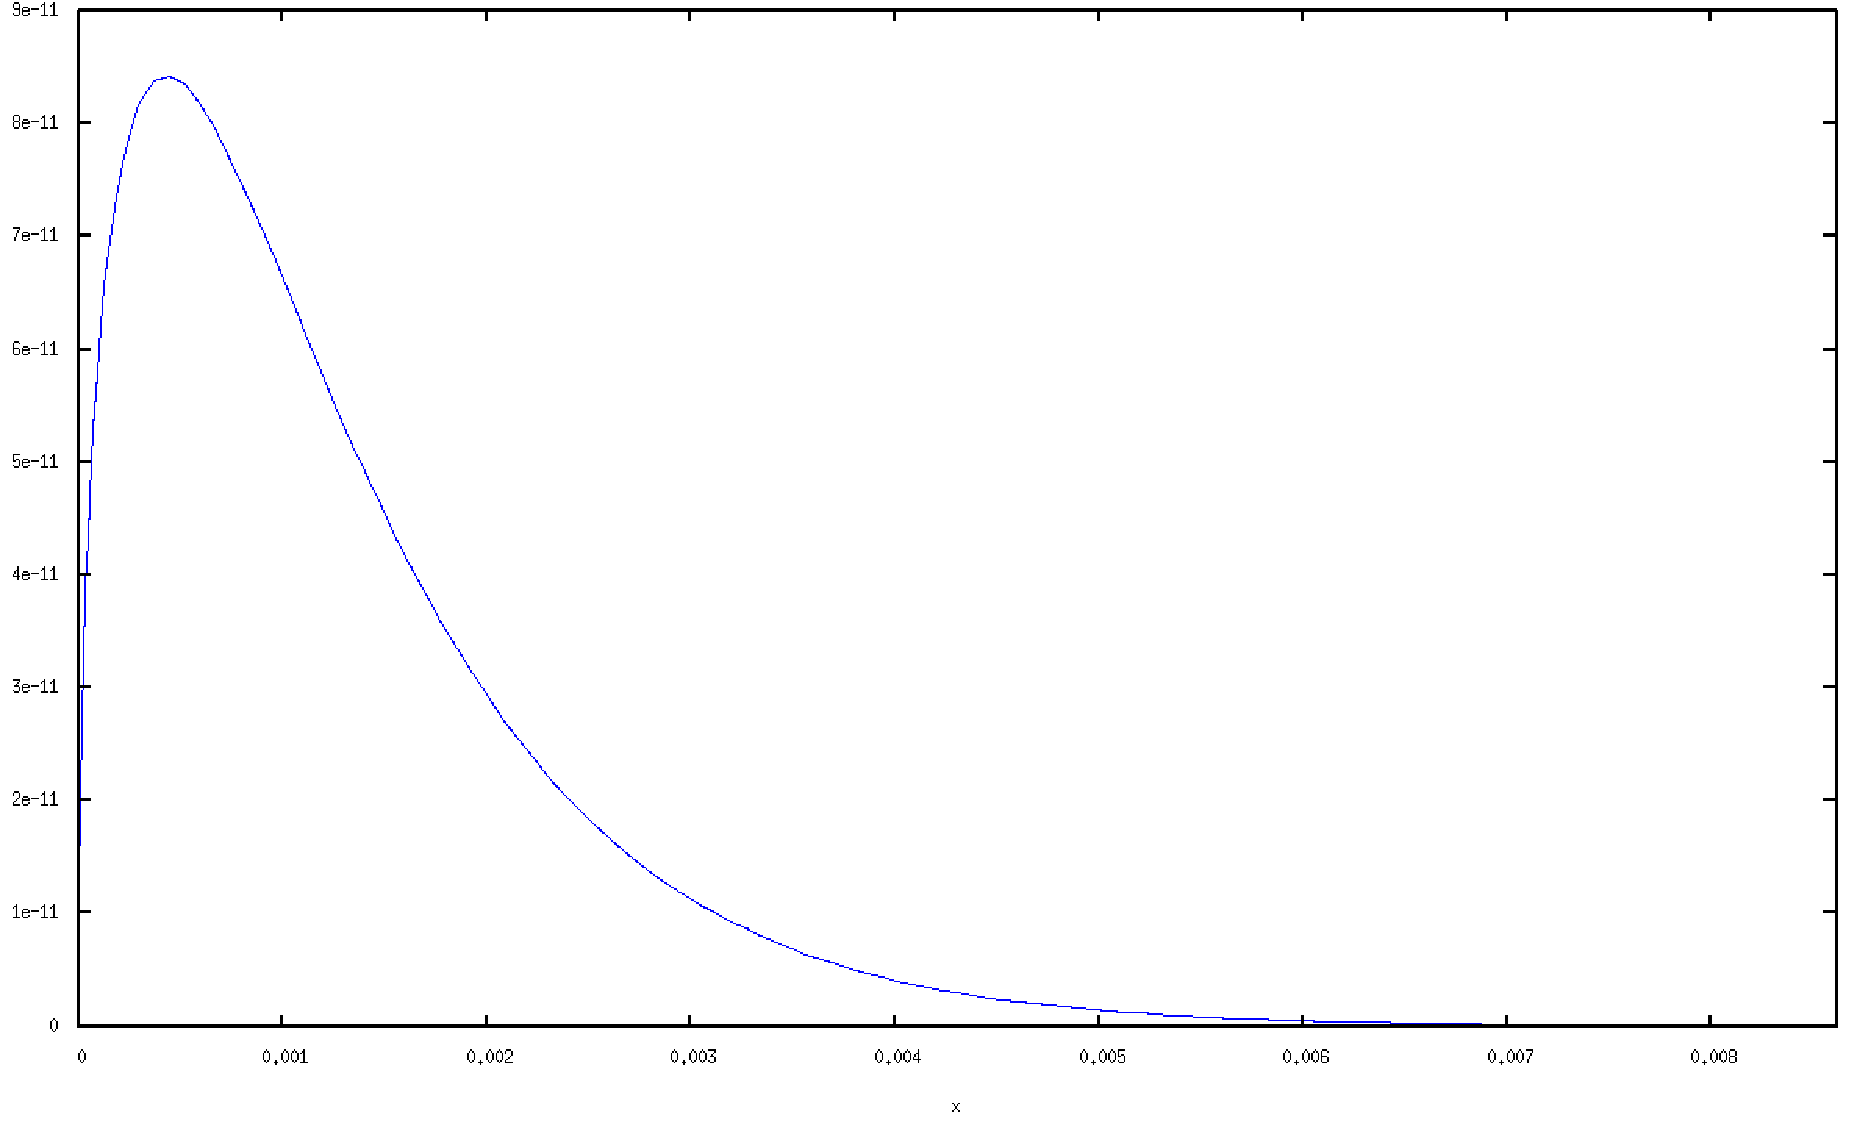
\includegraphics[width=0.30\textwidth]{04.pdf}
\caption{O gráfico mostra a distribuição de energias para um certo gás.}
\label{04}
\end{figure}
\
\noindent{\bf Questão 5-)} Nessa questão o objetivo na primeira parte foi utilizar o comando solve para encontrar as raízes do polinômio $f(x)=(3+x)^{2}-12$ e depois plotar o gráfico da função para verificar se o resultado confere. Encontramos para a função f(x) as soluções $x=-2\sqrt{3}-3$ e $x=2\sqrt{3}-3$, que são valores que batem com o que é visto na figura \ref{05}. Na segunda parte utilizamos o comando solve para encontrar os autovalores do polinômio característico $p(\lambda)= \lambda^{3}-4(\omega_{0} \lambda)^{2}+10\omega_{0}^{4}\lambda-4\omega_{0}^{6}$ e encontramos exatamente os autovalores:
\begin{eqnarray}
\lambda &=& (2- \sqrt{2}) \omega_{0}^{2}\\
\lambda &=& (2+ \sqrt{2}) \omega_{0}^{2}\\
\lambda &=& 2 \omega_{0}^{2}
\end{eqnarray}

\
\begin{figure}[h]
\centering
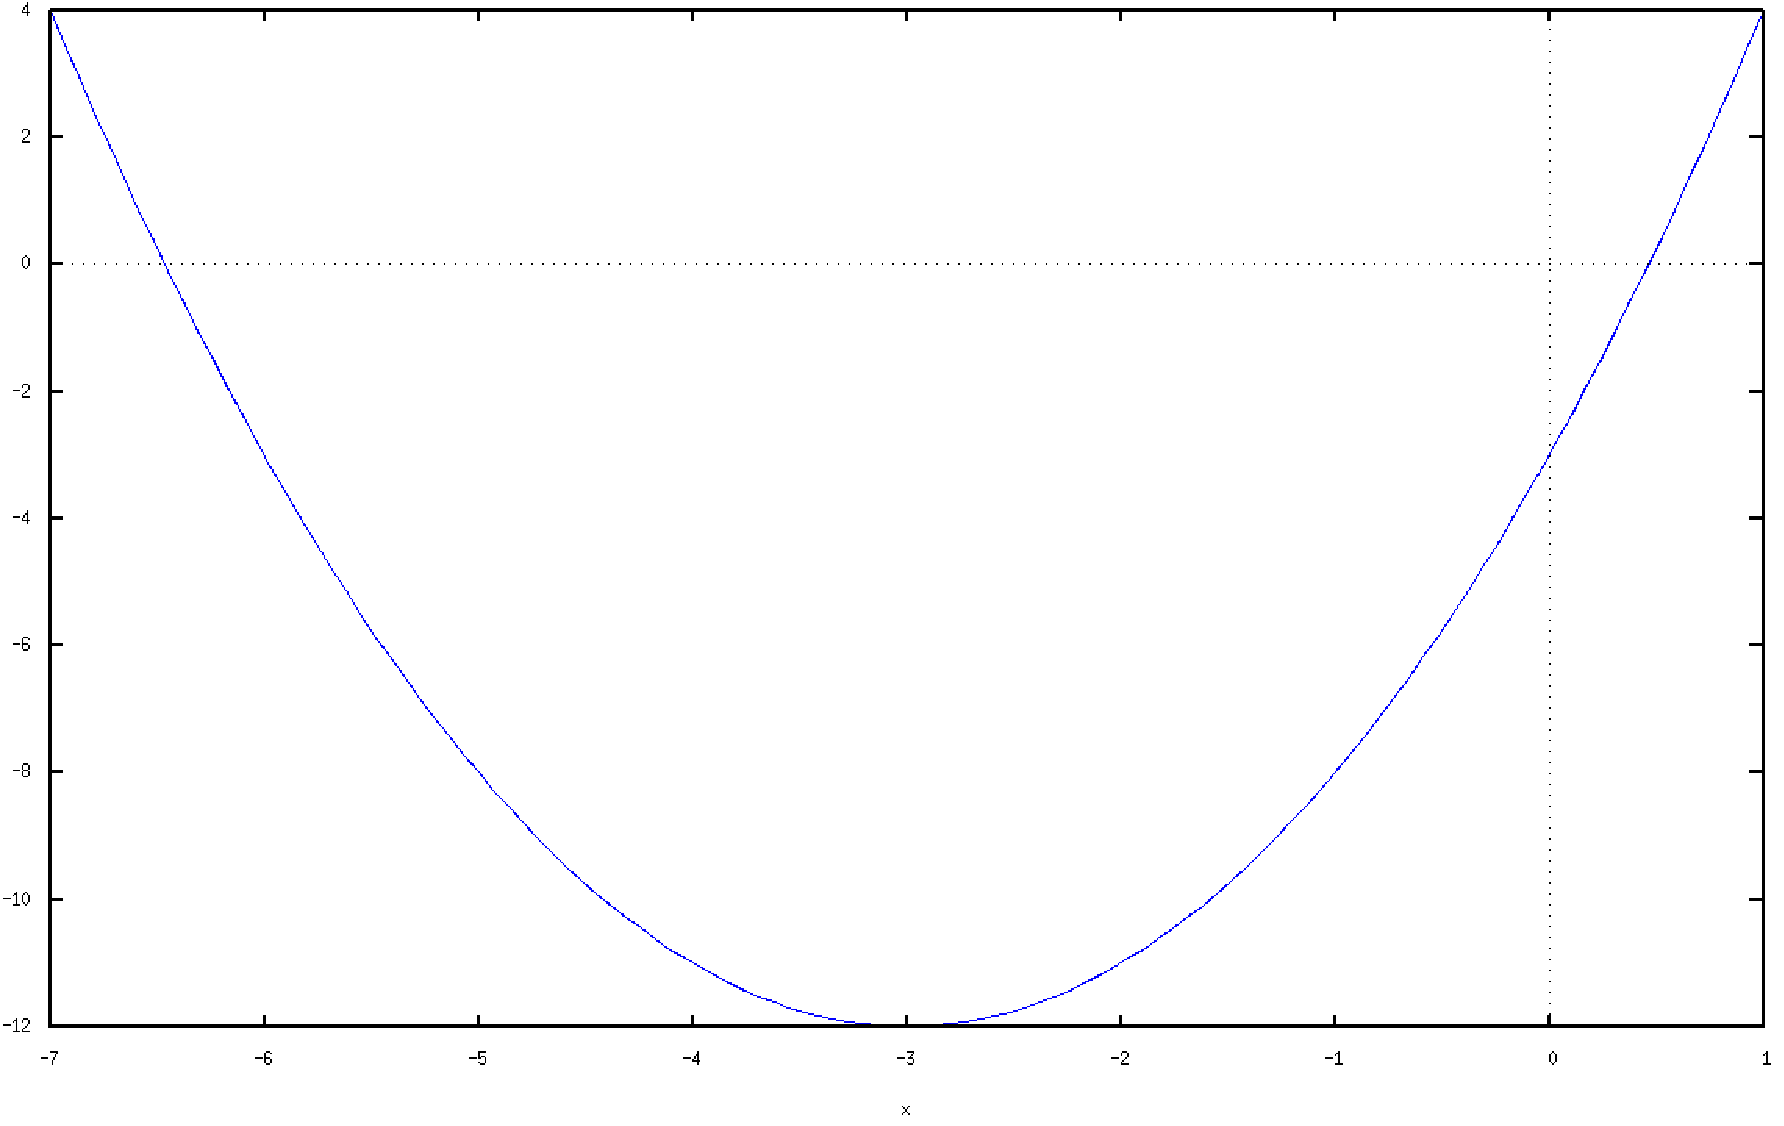
\includegraphics[width=0.30\textwidth]{05.pdf}
\caption{Gráfico da função $f(x)=(3+x)^{2}-12$.}
\label{05}
\end{figure}
\
\noindent{\bf Questão 6-)} O objetivo desta questão é utilizar o comando ode2 para encontrar a solução da edo $\dfrac{dy}{dt}=ry(1-\dfrac{y}{\kappa})$ e comparar com a solução que está no roteiro 7. Depois de seguir os passos do roteiro o programa quando foi executado imprimiu a seguinte relação:
\begin{equation}
-\dfrac{ln(y-\kappa)-ln(y)}{r}=-\dfrac{(-rt)-ln(y_{0}+ln(y_{0}-\kappa))}{r}
\end{equation}7
\
Aplicando a exponencial nos dois lados encontramos:
\begin{equation}
\dfrac{y-\kappa}{y}=\dfrac{e^{-rt}(y_{0}-\kappa)}{y_{0}}
\end{equation}
Por fim manipulando os termos de modo a deixar tudo em função de y explicitamente encontramos:
\begin{equation}
y=\dfrac{\kappa y_{0}}{y_{0}+e^{-rt}(\kappa - y_{0})}7
\label{solucaorot7}
\end{equation}
\
A equação \ref{solucaorot7} encontrada através do programa é a mesma que está exposta no roteiro 7, de modo que para essa edo a solução foi muito boa.
\

\noindent{\bf Questão 7-)} Nesse exercício alguns comandos foram utilizados para conhecer as ferramentas que tratam matrizes no maxima. O comando matrix foi utilizado para escrever as matrizes, R,i,V. O comando invert foi utilizado para inverter a matriz R e a notação de operações não comutativas de matrizes foi utilizada para fazer multiplicações, de modo que os seguintes resultados foram obtidos:
\[
R=
  \begin{bmatrix}
    r_{s} & r_{1} & r{2} \\
    -r_{x} & r_{1} + r_{x} + r_{a} & -r_{a} \\
    -r_{3} & -r_{a} & r_{2} + r_{s} +r_{a} 
  \end{bmatrix}
\]

\[
i=
  \begin{bmatrix}
    i_{1} \\
    i_{2} \\
    i_{3}
  \end{bmatrix}
\]
\\
\[
V=
  \begin{bmatrix}
   v_{0} \\
   0 \\
    0 
  \end{bmatrix}
\]


Assumindo os valores  $v_{0}=1,5 V,r_{1}=r_{2}= 100 \Omega, r_{3}=150 \Omega$ e $ r_{x}=120 \Omega $ e fazendo a seguinte operação não comutativa de matrizes no programa:
\begin{equation}
i=R^{-1}.V
\end{equation}
Encontramos a seguinte matriz i:
\[
i=
  \begin{bmatrix}
   0,012013729577167 \\
   0,006864988558352403 \\
    0,006933638443935927
  \end{bmatrix}
\]


\end{document}
